% template d'article LaTeX créé par Max De Wilde (STIC - ULB)
% contact : madewild@ulb.ac.be
% modifié par : Selim Ben Ismail
\documentclass[a4paper,12pt]{report} % ce document est un article sur une feuille A4, police taille 12
\usepackage[utf8]{inputenc} % encodé en utf-8
\usepackage[T1]{fontenc} % compatible avec les accents
\usepackage[french]{babel} % rédigé en français
\usepackage[hyphens]{url} % formatte les liens en autorisant la césure au niveau des traits d'union
\usepackage[pdftex,urlcolor=black,colorlinks=true,linkcolor=black,citecolor=black]{hyperref} % liens cliquables mais non colorés
\usepackage[top=3cm,bottom=4cm,left=4cm,right=2.5cm]{geometry} % gère les marges
\usepackage{graphicx} % gestion des images
\usepackage{array} % gestion des tableaux
\usepackage{csquotes} % gestion des guillemets
\usepackage{longtable}
\usepackage{colortbl}
\usepackage{xcolor}
\setlongtables
\usepackage{fourier} % utilise une autre police que celle par défaut (Computer Modern)
\usepackage[absolute]{textpos}
%Chapter form
\RequirePackage[Sonny]{fncychap}
\usepackage{setspace}
%\setstretch{1,5} % définit l'interligne
%\setlength{\parskip}{0,5cm} % définit l'espacement entre paragraphe
\usepackage[             % bibliographie
   backend=biber,        % compilateur par défaut pour biblatex
   sorting=nyt,          % trier par nom, année, titre
   citestyle=authoryear, % style de citation auteur-année
   bibstyle=alphabetic  % style de bibliographie alphabétique
]{biblatex}
\addbibresource{biblio.bib}
\AtEveryCitekey{\clearfield{note}\clearfield{pages}\clearlist{location}\clearlist{publisher}\clearfield{doi}\clearfield{url}\clearfield{urlyear}}

\usepackage{chngpage}
\usepackage{amsmath}
\usepackage{footnote}
\usepackage{appendix}
\usepackage[nottoc]{tocbibind}
\usepackage{pdfpages}

\begin{document}
%page de garde

\begin{titlepage} % style spécial pour la page de garde
%\singlespacing % remet l'interligne normal pour cette page
\begin{center} 
\huge{\textsc{Université Libre de Bruxelles}}\\
\vspace{.5cm}
\LARGE{Faculté de Lettres, Traduction et Communication}
\end{center}

\vfill % laisse LaTeX gérer l'espacement vertical

\begin{center}
\Huge{Cartographie sur base d’exploration des données automatisée de documents en langue ancienne}\\ %titre ici
\vspace{.5cm}
\LARGE{étude du cas de Douai au XIIIe siècle} %sous-titre
\end{center}

\vfill

\begin{tabular}{b{5.5cm}b{7.5cm}} % taille et alignement des cellules du tableau
Selim \textsc{BEN ISMAIL} & Mémoire présenté sous la direction de Sébastien \textsc{DE VALERIOLA} en vue de l'obtention du titre de Master en Sciences et Technologies de l'information et de la Communication\\ % ajoutez vos nom et prénom ainsi que ceux de votre directeur de mémoire
\end{tabular}
\vfill
\begin{center}
Année académique 2021--2022 % vérifiez que l'année est correcte !
\end{center}
\end{titlepage}

\newpage
\chapter*{Résumé}
 Ce mémoire de recherche détaille la conception d’un système dont l’ambition est de produire des cartographies de la ville de Douai à l’époque du XIIIe siècle, sur la base de données acquises par une fouille de texte automatisée au travers du registre de rentes de Sire Jehan de France.
 Trois thèmes majeurs sont au centre de ce travail de recherche : l’application des outils de traitement automatique des langues naturelles (TALN) aux documents historiques, l'application d'analyse de réseaux, et la visualisation des données par la cartographie 
 
\vspace{0.5cm}
\textbf{\textit{Mots-clés : Douai, TALN, Analyse de réseaux, Jean de France, Cartographie}}



\newpage
%remerciements
\chapter*{Remerciements}

\setlength{\parskip}{0,5cm}% set l'espace entre les paragraphes

Par la rédaction de ce mémoire s'achève mon parcours académique au sein de l'Université Libre de Bruxelles.
Ce chemin fut long et éprouvant  mais  incroyablement riche en apprentissages et en rencontres.

S'il est une leçon que je retiendrai de celui-ci, c'est que la réussite n'est jamais l'accomplissement d'une unique personne. Je tiens donc à adresser des remerciement très sincères à certaines de celles qui m'ont permis d'arriver là où j'en suis.

Tout d'abord, à mon promoteur de mémoire , Monsieur Sébastien De Valeriola. Pour m'avoir suivi, guidé, et encouragé, tout au long de ce travail. 

Ensuite, à Lidia Mantesso, Edouard Vaché, David Manfroy, Eléonore Bastogne, quatre étudiants qui ont partagé mon périple universitaire. Depuis les premiers cours de passerelle, jusqu'aux derniers de master, nous nous sommes entre-aidés et soutenus, jusqu'à devenir des amis, au delà de nos études.

Je voudrais également remercier les personnes qui partagent mon quotidien et me supportent, jour après jour. Mes parents, Véronique Doms et Mehdi Ben Ismail, mes colocataires, Réjane Janzyk et Corentin Dardenne. 

Et finalement, Primus, le chat de ma colocataire, qui veilla tant de soirs à mes côtés. Merci pour tes ronronnements réconfortants.

\setlength{\parskip}{0cm}% set l'espace entre les paragraphes

%table des matières
\setstretch{1,5}
\tableofcontents
\newpage
\strut % ou ~ ou \mbox{} ou \null
\newpage
\setlength{\parskip}{0,5cm}% set l'espace entre les paragraphes

%introduction
\chapter{Introduction}
\section{Introduction générale}
 Ce mémoire détaille la conception d’un système dont l’objectif est de cartographier la ville de Douai à l’époque du XIIIe siècle sur la base de fouille de texte automatisée à travers un registre de rentes d'époque, celui de Jehan de France, un riche marchand drapier et patricien de la ville de Douai. Trois thèmes majeurs des sciences de l'information et de la communication sont au centre de cette recherche :
 
 La première thématique est l’application des outils de traitement automatique des langues naturelles (TALN) aux textes historiques. L’émergence des humanités numériques a ouvert la recherche en sciences humaines à de nouvelles méthodes d’analyses qui ont, depuis, déjà grandement prouvé leur efficacité. Cependant, dans le cadre de l’étude de textes historique, les outils utilisés par celles-ci se heurtent à de lourdes complications. L’une des principales est le langage dans lequel sont écrits des textes historiques : les outils de fouilles de textes sont généralement conçus pour traiter les langues très représentées telles que l’anglais ou le français et non des langues anciennes. Pour cause, une grande partie de ces outils ont besoin de corpus de textes conséquent ou de dictionnaires pour être performants. Un facteur accentuant cet état de fait est qu’il est relativement compliqué de composer un corpus de textes historiques : d’une part, parce que les textes anciens, étant sur des supports physiques, doivent être numérisés et ocrisés avant de pouvoir être utilisés, et d’autre part, car les sources écrites sont régulièrement lacunaires ou amputées d’une partie de leur contenu. La personne cherchant à traiter de façon automatisée des textes historiques devra donc se montrer créative.
 
La seconde thématique est l’application de la théorie des graphes au domaine de l’Histoire. La théorie des graphes trouve ses premières origines dans les travaux du mathématicien Leonhard Euler en 1735 et son problème des « sept ponts de Königsberg »\parencite{euler_solutio_1735}. Les graphes permettent de modéliser des problèmes complexes sous la forme d’une structure de sommets reliés entre eux par des arêtes où les sommets renvoient à des référents — cela peut être des personnes, des lieux, des propositions, etc. — et les arêtes aux relations qui les relient entre eux. Si la théorie fut d’abord utilisée pour résoudre des problèmes de géométrie ou de mathématique, elle s’est popularisée dans le domaine des sciences humaines dans les années 1960 afin de modéliser diverses problématiques.

Finalement, la troisième thématique est celle de la visualisation des données sous forme de cartographies. L’intérêt de la cartographie dans la recherche en Histoire est multiple. Le premier est que ces cartes sont la représentation d’un grand nombre de données agrégées. Elles permettent donc d’analyser des phénomènes déjà connus d’un point de vue plus éloigné et plus global, permettant ainsi de découvrir de nouvelles relations corollaires ou causales entre différents évènements qui ne semblaient pas forcément liés aux premiers abords. À l’instar de l’exploration de graphiques et données statistiques, l’exploration des différents types de cartes se pose comme une approche complémentaire à l’étude des sources primaires dans les recherches en Histoire.

Un autre intérêt majeur de la visualisation des données se trouve dans la communication et la transmission des savoirs. En effet, l’information visuelle, pour peu qu’elle soit correctement organisée et présentée, s’appréhende et s’assimile avec plus d’aisance que l’information textuelle brute. Or c’est dans cette transmission que l’étude de l’Histoire prend son plein sens.

\section{Question de recherche}
 La question de recherche est \emph{\og La théorie des graphes, appliquée au domaine des patrimoines immobiliers en Flandre médiévale, couplée à une fouille de texte automatisée dans des textes historiques, permet-elle de produire des visuels cartographiques pertinents à l’étude de l’histoire urbaine ?\fg{}} 
 
 Derrière cette question de recherche relativement vaste, se dissimule en réalité l'évaluation du résultat de trois objectifs distincts mis bout à bout. À savoir : développer des algorithmes de fouille et traitement de textes adaptés à un document historique, appliquer la théorie des réseaux aux résultats obtenus par cette fouille afin de représenter des liens de mitoyennetés, et finalement, transposer ces graphes en un visuel cartographique afin d'ouvrir de nouvelles voies de recherche dans l'étude du développement urbain.
 
\section{Hypothèse}
Le mémoire présente un travail de recherche et la conception d'un prototype, d'un \textit{proof of concept} permettant de répondre à la question de recherche. Très peu de travaux, si ce n'est aucun, n'ont été publiés sur cette méthode d'analyse des documents médiévaux. Il est donc difficile d'émettre des hypothèses quant aux limites qui seront rencontrées et sur les résultats qui seront obtenus.

Toutefois, cette méthode semble réalisable dans la théorie, et dans une optique optimiste,  les visuels produits devraient permettre de rendre compte des propriétés immobilières de Jehan de France, de la disparité et des types des loyers en fonction des quartiers de la ville, de la dispersion des noms de famille, etc. Des éléments qui, croisés  à d'autres sources, pourraient valider ou invalider d'autres hypothèses. 



\section{Contexte historique}
\subsection{La ville de Douai au XIIIe siècle}

Douai trouve ses origines au VIe siècle sur un îlot de la Scarpe (\cite{mestayer_douai_2016}), une rivière traversant le nord de la France et se déversant dans le fleuve de l'Escaut. Les terres fertiles des alentours offrent une rapide croissance à ce qui n'est alors encore qu'une petite agglomération rurale. Dès le Xe siècle, l'agglomération s'étend sur les rives de la Scarpe. Au nord, sur la rive gauche de la rivière, le \textit{Duaculum}, appelé aussi le \textit{Douayeul}, une zone rurale dépendant de l'église Saint-Albin comprenant élevages de bêtes, greniers et brasseries (\cite{mestayer_douai_2016}). Sur l'autre rive, au sud, le \textit{Castel Bourgeois}, un quartier qui s'oriente davantage vers le commerce et l'artisanat. Ce dernier deviendra la première place marchande de la ville (\cite{netteghem_histoire_2021}). En 967, Douai, qui à cette époque est encore appelé \textit{Castrum Duacum}, se dote d'une place forte ainsi que d'une première muraille entourant la partie haute et basse de la ville (\cite{mestayer_douai_2016}). 

Forte de son activité agricole et de ses accès fluviaux, la ville gagne en richesse et devient un centre de commerce important dans la région qui attire marchands et artisans(\cite{clisant_vie_2003}). Les quartiers de la ville s'organisent alors en fonction des rassemblements d'artisans et marchands. On retrouve par exemple la rue des ferronniers, des foulons ou encore des bouchers. Les rues et places prennent à cette époque, où le pragmatisme  prévaut, une dénomination en fonction de leurs usages \cite{colin_decouvrez_2001}). 

Au XVIIe siècle, la disparité entre les deux rives se fait de plus en plus clivante et donne l'impression d'une ville séparée en deux entités distinctes (\cite{leroy-langelin_quartier_2012}). 
Le centre névralgique de la ville se consolide sur la rive droite de la Scarpe : une seconde enceinte, comportant douze portes, est édifiée afin d'englober l'expansion des quartiers autour du \textit{Castel bourgeois}, où des places de marchés ainsi que des halles apparaissent. 
Si le commerce céréalier fit démarrer la machine économique de la cité, Douai se forge maintenant une réputation, principalement, autour du commerce de draperies. Grâce aux foires de Champagne, la draperie douaisienne s'exporte à travers à toute l'Europe, et même au-delà (\cite{clisant_vie_2003}). Ce succès provient de la qualité et de la finition des étoffes produites, foulées aux pieds pour les plus précieuses. Chaque étape de la fabrication était supervisée par une des grandes familles bourgeoises de Douai (\cite{clisant_vie_2003}).
La progression économique que connait la ville grâce au commerce de draperies est très liée à la production agricole des campagnes avoisinantes, car ces dernières fournissent la matière première à cette nouvelle industrie.
Cependant, rapidement, la production de laine locale ne suffit plus à combler la demande en étoffes et un commerce s'installe avec l'Angleterre qui approvisionne alors Douai en laine(\cite{clisant_vie_2003}).

À la fin du XIIe siècle, un premier échevinage apparaît, constitué de douze riches et notables douaisiens (\cite{mestayer_douai_2016}. Ceux-ci régissent les activités, ainsi que les affaires financières, policières et juridiques de la ville au moyen de bans : une forme d'arrêté législatif (\cite{verriest_espinas_1914}). Ceci témoigne de la place, de plus en plus importante, qu'occupent les grandes familles bourgeoises dans l'administration et le développement de la ville.

Au cours de l'Histoire, Douai ne cesse d'être, tantôt française, tantôt flamande. Cependant, la richesse et la puissance de la ville font qu'elle garde toujours une certaine indépendance vis-à-vis du roi de France ou du comte de Flandre dans son administration (\cite{mestayer_douai_2016}).

La construction d'un nouveau rempart est entreprise au XIIIe siècle, justifié par l'apparition de nouveaux quartiers extérieurs à la seconde enceinte, tels que la \textit{Neuville} au  nord ou le \textit{Faubourg de Notre-Dame} à l'Est (\cite{netteghem_histoire_2021}).
Parallèlement à l'apogée économique de la ville, une nouvelle forme de marché\footnote{Ou de \og capitalisme \fg{} comme l'appelle G.Espinas (\fullcite{espinas_les_1933})} émerge : l'hiterage, qui recouvre toutes les formes de la propriété bâtie, y compris les terrains et les rentes de celles-ci. Ces bourgeois, principalement marchands et disposant déjà d'une certaine fortune mobilière, cherchent alors à acquérir biens-fonds et rentes ; un patrimoine qui devient un gage d'honorabilité et un signe de réussite dans la cité  (\cite{leguay_propriete_1989}). 

\begin{figure}[ht] % insère une figure ici (h = "here")
    \centering
    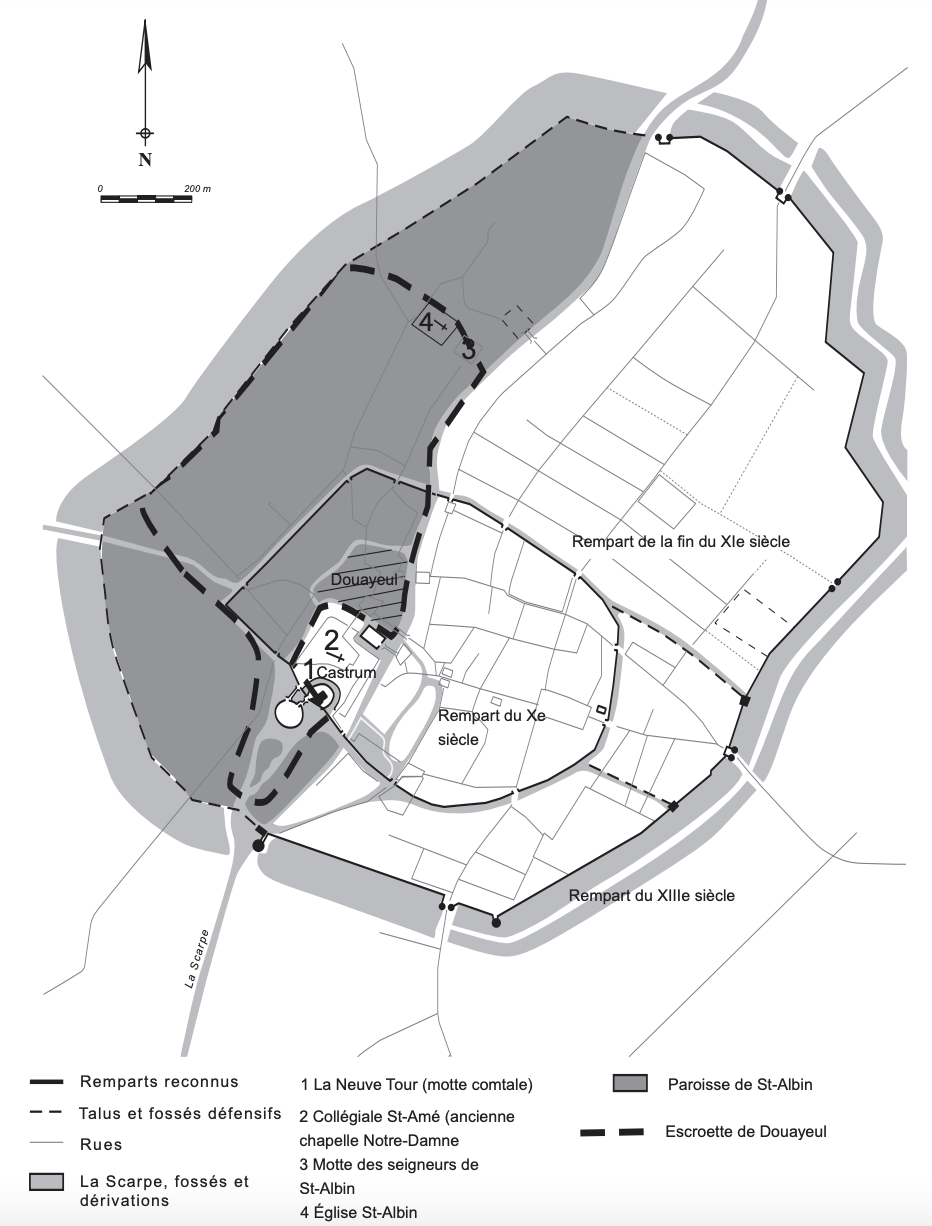
\includegraphics[scale=1]{1.Introduction/Img/Plan général de la ville de Douai avec les enceintes successives. DAO : E. Leroy-Langelin.png} 
    \caption{Plan général de Douai au XIIe s., E.Leroy-Langelin}
\end{figure}

\subsection{Sire Jean de France}
Sire Jean de France\footnote{On retrouve différentes graphies de cet anthroponyme, tel que \og Jehan de France\fg{} ou \og Jehans de Franche\fg{}, pour autant, il s'agit du même personnage. Cette pluralité de graphies des anthroponymes affecte également ses contemporains et sera traitée plus loin, dans le chapitre \textit{Méthodes}} est un bourgeois notable de Douai qui vécut dans la seconde moitié du XIIIe siècle. Il est, marchand drapier, propriétaire immobilier, à plusieurs reprises, échevin, par quelquefois, prêteur d'argent, notamment pour les comtes de Flandre, mais surtout patricien (\cite{espinas_les_1933}). 
Mais malgré ses titres à Douai et son patrimoine immobilier (estimé à 316 rentes sur 529 maisons , ainsi que quelques propriétés hors de la ville (\cite{blockmans_trois_1941})) on retrouve finalement assez peu de travaux de l'historiographie de ce personnage, resté dans l'ombre d'autres patriciens de Douai de la même époque.

Les dates de naissance et de mort de Jean de France ne sont pas connues avec exactitude, mais les premières traces de son existence remontent à 1252 et sa mort est supposée en 1298 (\cite{espinas_les_1933}). Nous savons qu'il avait comme mère Heluys, qui , par ailleurs, lui légua sa première rente\footfullcite[p.3]{espinas_les_1933}
On sait également qu'il  avait deux frères : Jakemes et Pieres et qu'il a eu au cours de sa vie, une fille, Hielotain, qui devint abbesse du monastère de Sin-le-Noble. En revanche, il n'a été retrouvé aucune mention de son père (\cite{espinas_les_1933}).

Le régime patricien, fut caractérisé par une exploitation de la misère, principalement celle des ouvriers et des universitaires (\cite{blockmans_trois_1941}). La figure la plus emblématique de patriciat est sans doute Jehan Boinebroke  que Fr. Blockmans nous décrit comme tel :
\begin{displayquote} 
    \og J. Boinebroke apparaît comme l'incarnation d'un capitalisme tellement hideux, si cruel et si impitoyable, que même la première moitié du xixe siècle n'en a pas connu de pareil ! \fg{}\footfullcite[p. 266]{blockmans_trois_1941}
\end{displayquote}
\vspace{0,5cm}
À son opposition, Jean de France est dépeint par G. Espinas et Fr. Blockmans comme un investisseur prudent et plutôt bienveillant :
\begin{displayquote}
    \og [...] il représente d’une façon directe une forme de capitalisme foncier sortie de la propriété immobilière. Cependant, ce n’est pas un égoïste..Il a pu jouir de son argent, de ses revenus pour lui-même, mais il ne les a pas gardés exclusivement pour lui, il a pensé aux malheureux, aux « déshérités de la vie » et sans doute, mù expressément par une pensée religieuse, il a fondé en leur faveur une institution de bienfaisance : il s’est montré un riche charitable.\fg{} 
    \footfullcite[p.139]{espinas_les_1933} — G. Espinas
\end{displayquote} 
\vspace{0,5cm}
D'ailleurs, lors des insurrections du peuple antipatriciennes qui frappèrent Douai à la fin du XIIIe siècle, le nom de Jean de France ne figura pas sur la liste des bannis malgré son appartenance indéniable à l'élite bourgeoise de la ville(\cite{espinas_les_1933}).

\subsection{Registre de rentes de Jean de France}
Le registre de rente de Jean de France, ou pour reprendre du document même, \textit{l'escris}, est un document d'origine privé, écrit en picard médiévale, déposé à l'hospice des Chartriers de Douai en octobre 1291. 

Le document recense toutes les rentes de Sire Jean de France à la date du dépôt (octobre 1291). Celles-ci sont classées par ordre topographique selon les \textit{escroetes} (\cite{espinas_les_1933}). Les \textit{escroetes} sont au nombre de six et divisent la ville en quartiers. Elles sont : \textit{li escroete dou Markiet}, \textit{li escroete de Canteleu}, \textit{li escroete dou Més}, \textit{li escroette des Wés}, \textit{li escroete de Douayeul}, \textit{li escroete de Neuville}.
Ces \textit{escroetes}, sont elles-mêmes divisées en sous-éléments topographiques correspondant la plupart du temps aux connétablies. Il peut s'agir de rues, de places, de porte, etc. Finalement, s'il s'agit de rues ou de places importantes, ces subdivisions sont encore une fois divisées en fonction du \textit{rench}, correspondant au rang de la voie.

De par sa complétude et son écriture, qui ne comporte que très peu d'imperfections et d'irrégularités, cet ouvrage est particulièrement précieux pour approcher le contexte économique et social de l'époque. 
Toutefois, il faut pouvoir appréhender cette source de la manière dont il conviens : certains éléments sont obscures ou donne lieu à des interrogations. Pour cause, il s'agit là d'un document de résultats et non de formation (\cite{espinas_les_1933}).

L'utilisation du registre prend toute sa pertinence dans nos recherches, car chaque entrée contient, non seulement le nom du débirentier
%\footnote{\og Personne qui doit une rente.\fg{} définition du dictionnaire Larousse, consulté à la date du 26/09/2022 https://www.larousse.fr/dictionnaires/francais/d\%C3\%A9birentier/21806} 
et le montant, ainsi que le type de la rente, mais également une indication sur la localisation de la propriété. Cependant, cette information est donnée de manière indirecte en citant le nom des habitants des propriétés voisines, ou dans de rares cas, les éléments topographiques adjacents comme une porte (d'enceinte), une place ou une chapelle.

%méthodes
\chapter{Méthodes}
Les étapes au sein du processus défini pour passer du registre de rentes en format texte (\textit{.txt}) en cartographie de la région de Douai peuvent être classées en trois types distincts : les opérations d’extraction, les opérations de traitement et les opérations d’exploitation. Il ne s’agit pas, là, de trois phases , comme intuitivement nous pourrions le supposer, mais de trois classes d'opérations qui s’alternent en fonction des étapes du processus.

\section{Le document source}
Il faut, tout d'abord, évoquer le document source qui sert, non seulement, d'entrée au système, mais comme  il sera vu plus tard\footnote{c.f. Sous-chapitre de l'extraction de l'information}, il servira également au développement et à l'évaluation du système.

Étant donné la préciosité et la fragilité matérielle du registre des rentes de Jean de France en tant qu'objet et les difficultés d'accès au document,il est évident que le travail n'a pas été exécuté directement à partir de celui-ci. Et, au regard de la calligraphie originale\footnote{un extrait est consultable dans les annexes}, presque heureusement, car cela aurait rajouté un travail important d'\textit{OCRisation} et de correction post-traitement. 
George Espinas, dans son second tome des \og Origines du capitalisme \fg , de 1936, a retranscrit dans une typographie plus actuelle l'intégralité du rentier de Sire Jean de France. C'est sur cette base\footnote{Pour être plus exacte, j'ai reçu de M. De Valeriola un document word(\textit{.docx}) contenant une une retranscription du registre déjà  grandement nettoyée des erreurs d'OCR et épurée d'une partie des symboles d'éditions qui complexifient l'utilisation des  outils de TALN} que le travail s'est effectué.

Le document comporte deux types de marqueurs que je définis comme tels : d'une part, les marqueurs d'éditions, qui sont les marques et symboles dus à l'édition du document (numéros de page, de ligne, de folio, de cahier, références de bas de page, etc.) et d'autre part, les marqueurs de structures, marques et symboles qui viennent directement du document et qui servent à l'organisation du texte (titres, sous-titres, etc.).

Dans le cas de notre document source, comme expliqué en bas de page, les marqueurs d'édition sont inexistants à l'exception des numéros de page\footnote{ Il s'agit des numéros de page provenant du livre de G.Espinas, interrompant le texte là où c'était le cas dans ledit livre}. Quant aux marqueurs de structure, on retrouve :
\begin{itemize}
\item le numéro d'escroete marqué par un chiffre romain et suivi aux lignes suivantes d'une définition.
\item le numéro de connétablie marqué par un caractère \og ° \fg et éventuellement d'un second numéro ou d'une mention \textit{bis}, suivi d'une définition sur les lignes suivantes.
\item Les marqueurs de rang de voie de la connétablie, indiqués par les caractères \og A \fg et \og B \fg.
\item Les numéros de rentes successives et de rentes successives dans une même connétablie. Le second numéro vient en exposant du premier dans le document original de G.Espinas, mais lorsque celui-ci est transformé en format texte (\textit{.txt} pour être traité par le logiciel \textit{R}, le codage de l'exposant n'est plus pris en compte et les deux numéros se concatènent. Ce problème sera détaillé plus en profondeur dans le chapitre \textit{Résultats}.  
\end{itemize}











\section{Extraction de l'information}
L'extraction se compose des phases de segmentation du texte, de la reconnaissance des entités nommées (REN), de l'analyse des relations entre entités. Toutes les étapes qui extraient, d'une manière ou d'une autre, de l'information depuis le document source ou d'un fragment de celui-ci. 
La finalité des opérations d'extraction de l'information dans le cadre de ce processus est de fournir un tableau de données, ou un système de table de données, reprenant toutes les informations semi-structurées du document source mises sous forme structurée, de sorte que ces données puissent directement servir à des études quantitatives.

\subsection{Segmentation du texte}
La segmentation du texte est l'une des premières phases du processus. Comme préalablement expliqué, les rentes sont ordonnées dans le registre en fonction d'éléments topographiques (escroete, connétablie, rang de voie) et chacun de ces éléments topographiques est renseigné par un marqueur de structure. Deux précisions  importantes : premièrement, les éléments topographiques représentés par ces marqueurs sont hiérarchisés; secondement, chacun de ces marqueurs de structure est unique\footnote{A l'exception des marqueurs de rang de voie.}.
Cela signifie, d'une part, que les rentes sont toujours situées dans une connétablie, elle-même située au sein d'une escroete et d’autre part, qu'une rente ne peut appartenir qu'à une et une seule connétablie, au même titre qu'une connétablie ne peut appartenir qu'à une et une seule escroete.
Le cas des indications du rang de voie est plus particulier dans le sens où selon la nature de la connétablie - qui n'est pas dans tous les cas, une rue ayant deux rangées de propriétés bâties - elle peut ne pas être présente et aussi parce que les rangs de voie, à la différence des autres éléments topographiques, ne disposent pas d'identification unique.
Les marqueurs des structures, étant chacun unique, ils constituent des clés idéales pour identifier une rente ou un groupement de rentes en fonction d'un élément topographique. 

C'est donc sur base de la reconnaissance de ces marqueurs par des \textit{regex}\footnote{appelées aussi \og expressions régulières\fg{}.} que l'algorithme va, de manière récursive, découper le texte initial en plusieurs parties. Dans un même temps, l'algorithme va construire un tableau de données afin de  recueillir les informations. 

La figure 2.1 illustre par un organigramme les étapes effectuées par le script de segmentation du texte source.
L’algorithme va en premier lieu parcourir le fichier et indexer tous les marqueurs d'escroete. Pour chaque marqueur d'escroete indexé, la section concernant celle-ci, ainsi que la définition correspondante, va être capturée et stockée dans un tableau de données\footnote{appelé aussi \textit{dataframe}, ou \textit{df} en abrégé}. Maintenant que le document texte est découpé au niveau des marqueurs d'escroete, pour chaque escroete répertoriée dans le tableau de données, une fonction similaire est appelée  en prenant comme argument la section de l'escroete concernée au lieu du texte source.
La fonction appelée détecte et indexe les marqueurs de connétablie. 
Ensuite pour chaque marqueur de connétablie indexé, la section est capturée et stockée dans un nouveau tableau de données, où pour chacune des connétablies, à nouveau, une fonction similaire est appelée pour exécuter les mêmes opérations ( indexation des marqueurs, capture et stockage des sections ) au niveau des rangs de voie, puis encore une fois au niveau des rentes.

Une fois la section de toutes les rentes d'un rang de voie stockées dans un tableau de données avec leur clé
\footnote{La clé prend la valeur du marqueur, dans le cas des rentes il s'agit du numéro de rente}, 
la fonction appelée renvoie ce tableau à la fonction appelante. Soit la fonction d'extraction des rangs de voie, si la connétablie en possède, soit directement la fonction d'extraction des connétablies dans l'autre cas. La fonction appelante va collecter tous les tableaux - un pour chacune des sections qu'elle stocke dans son propre tableau de données - et va ensuite les fusionner en y rajoutant sa propre clé (indicateur du rang de voie ou numéro de connétablie). L'opération est répétée ensuite vers les fonctions appelantes supérieures.

De l'exécution du script résulte un tableau de données contenant la clé et la définition de chaque escroete, de chaque connétablie, et de chaque rente. La création d'un système de tables de données au lieu d'un grand tableau de données a également été envisagée, cependant la solution du tableau de données a été retenue pour sa plus grande simplicité de mise en place et d'utilisation pour et parce qu'elle était suffisante pour les besoins du projet. L'alternative du système de table de données sera abordée avec plus de précision  dans la partie \textit{Discussion} du mémoire.

\begin{figure}[ht] % insère une figure ici (h = "here")
    \centering
    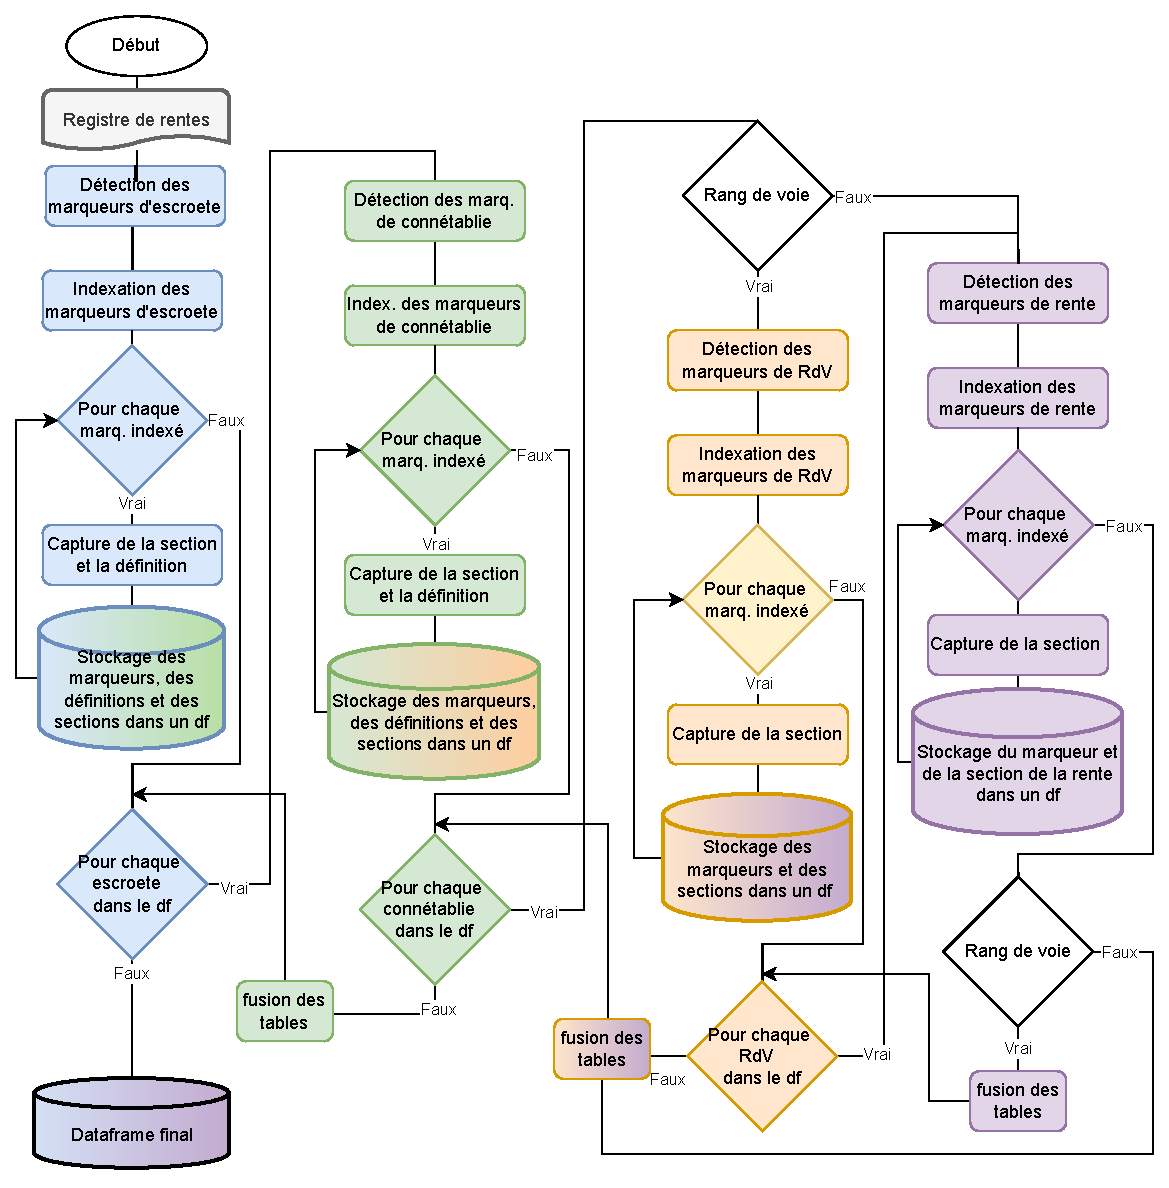
\includegraphics[scale=0.75]{2.Methods/Img/seg.drawio.pdf} 
    \caption{Organigramme de la segmentation automatisée du registre de rente.}
\end{figure}

\subsection{Reconnaissance et extraction des entités nommées}
Le concept d'\textit{entité nommée} désigne les unités textuelles possédant une fonction de référentiel au sein d'un contexte. Les noms propres, de personnes, de lieux, ou d'organisations, en sont l'exemple le plus évident, mais les entités nommées peuvent prendre bien d'autres formes telles que des pronoms, des valeurs numériques ou des descriptions définies \parencite{omrane_les_2010,nadeau_survey_2007}.

Selon le type d'entités nommées que l'on cherche à détecter et la nature du texte, la reconnaissance d'entités nommées peut s'avérer être une tâche complexe. Dans le cas de nos travaux, la reconnaissance d'entité se limite à la détection d'anthroponymes et de lieux (dit \textit{toponyme}) et ne s'avère par conséquent relativement pas trop complexe. Cependant, au vu des ressources possédées, ni les approches \textit{orientées connaissances}, utilisant des lexiques, ni les approches \textit{orientées données}, basées sur un apprentissage automatique,  ne sont exploitables. Il faut donc retourner à une  approche plus historique qui se concentre sur la reconnaissance de caractères morphologiques tels que les majuscules \parencite{nouvel_reconnaissance_2012}. 

La méthode utilisée se base intégralement sur les travaux de S. De Valeriola. Celle-ci conçoit les anthroponymes comme l'assemblage d'un  nom de baptême et d' un patronyme. Patronyme qui est constitué d'un ensemble d'unités textuelles  pouvant être rassemblées en  groupes de mots ayant la même structure. Plus concrètement, on retrouve, potentiellement,  une ou plusieurs particules  suivies d'un ou plusieurs \og noms \fg{}. La méthode combine donc trois expressions régulières afin de détecter ces trois éléments évoqués : le prénom, la ou les éventuelles particules liées au nom de famille et le ou les noms \parencite{de_valeriola_lordinateur_2021}. L'approche développée est évidemment spécifique aux anthroponymes du contexte historique décrit dans la partie \textit{Introduction}.

\subsection{Analyse des relations entre entités}
Rappelons, que dans ce contexte, les entités nommées sont presque uniquement des anthroponymes, et à de rares occasions, un lieu comme une porte d'enceinte ou une place de marché, et que les relations qui les unissent sont des liens de mitoyenneté.
L'analyse des relations entre entités nommées se fait une fois de plus à l'aide d'expression régulière. Les entrés du registre de rentes, si en tant que telles, sont des données textuelles non structurées, présentent néanmoins un certain formalisme dans leur construction. G. Espinas nous dit à ce propos : 
\begin{displayquote}
    \og Les énoncés des propriétés et de revenus se présentent selon des conditions et même dans des formes tout à fait analogues, à peu près identiques, qui peuvent se schématiser ainsi : « Sur la ou sur les maisons d’un tel et sur tout le tenement — ki fu a un tel, au besoin — , qui siet entre le tenement d’un tel et le tenement d’un tel — , ki, de part et d’autre, furent à un tel, au besoin — , dou fons de le terre, ou apries le fons de le terre, régulièrement, ou sans indication d’affectation par exception — , tant de rente de telle nature, d’un seul ou de plusieurs éléments ».\fg{}
    \footfullcite[p.113]{espinas_les_1933}
\end{displayquote} 
\vspace{0,5cm}
Pour extraire les entités nommées et définir leurs relations, nous pouvons segmenter le texte de la rente deux partie, de part et d'autre de l'expression \og \textit{qui siet entre} \fg{}. Nous récupérons ainsi, dans la première partie, le nom du débiteur, et dans la seconde partie, les noms de ceux avec qui le débiteur partage un lien de mitoyenneté.





\section{Traitement de l'information}
%intro%
Les étapes de traitement de l'information reprennent toutes les opérations qui, d'une manière ou d'une autre, analysent et modifient le contenu original du document source ou des informations extraites. Il peut s'agir d'audit de la qualité des informations contenues dans un tableau, de la mise en place de contraintes d'intégrité, de corrections de données ou encore de regroupements de données. 
L'objectif des opérations de traitement de l'information est d'améliorer la qualité des données extraites afin qu'elle soit utilisable dans les opérations d'exploitation des données décrites dans la section suivante.

\subsection{Analyse de la qualité des données}
% définition des critères de qualité
S'il n'existe pas de consensus sur la définition même de ce que représente la qualité des données, pour autant, on peut s'accorder à dire que la qualité des données se décompose en une pluralité de critères dont la pertinence et le poids varient selon le cadre d'utilisation des informations \parencite{berti-equille_qualite_2004}. De ce constat, est né le concept \textit{fitness for use} qui dit que :
\begin{displayquote}
    \og La qualité de l'information ne renvoie jamais à la perfection de celle-ci, mais à son adéquation relative à un ensemble de besoins donnés. La tolérance à l'erreur variera en fonction des enjeux.\fg{} 
    \footfullcite[p.7]{boydens_delivrable_2007} 
\end{displayquote} 
\vspace{0,5cm}

%enjeux de la qualité dans les process automatisés
Cette qualité des données est un aspect critique dans tout processus d'automatisation. C'est particulièrement vrai lorsque plusieurs opérations automatisées se succèdent sans vérification de l'agent humain. De petites erreurs en début de processus peuvent alors se propager et prendre de l'ampleur à travers chacune des étapes suivantes. 

%exemple
Si, par exemple, à la suite d'une erreur, une escroete n'est pas détectée par l'algorithme de segmentation et n'est, de facto,  pas non plus répertoriée. De cette seule erreur, il découlerait qu'aucune connétablie située au sein de l'escroete ne serait alors répertoriée. Par extension, toutes les rentes situées dans ces connétablies seraient également non indexées et omises dans la suite du processus. Ainsi, une unique erreur peut finalement lourdement impacter les résultats obtenus en sortie du système.

%stratégie globale 
Afin d'éviter cela, des audits de la qualité des données récoltées ont été menés pendant la conception du système. En fonction des résultats rendus, les algorithmes ont été corrigés afin d'intégrer des contraintes d'intégrité (approche préventive) et des opérations de nettoyages des données(approche curative).
Dans le cas d'un système qui serait alimenté par des flux de données nouvelles, les phases d'audit devraient être intégrées au système lui-même ; on parlerait alors de \textit{gestion des processus} \parencite{berti-equille_qualite_2004}. Mais, dans le contexte qui est le nôtre, les données sont finies, plus aucune nouvelle entrée ne sera ajoutée au registre de rentes, on peut donc sortir les phases d'audit du fonctionnement du système et les cantonner au développement du système.

\subsection{Nettoyage des données}
%définition 
Le nettoyage des données est un processus d'amélioration des données qui a pour but, au travers d'une série de transformations, de normaliser les données et de détecter lorsque plusieurs enregistrements font référence à un même objet (phénomène de surcouverture) \parencite{berti-equille_qualite_2004}.

%stratégie de nettoyage %
Les stratégies pour la correction des données erronées sont aussi diverses que les causes d'où ces erreurs peuvent provenir. C'est pour cela qu'avant toute chose, il est impératif de comprendre la nature du document source et des données qu'il contient. Il faut pouvoir supposer les différents facteurs qui auraient pu altérer l'information lors de son inscription dans le document source afin de mettre en place les vérifications nécessaires pour anticiper, et le cas échéant, corriger les erreurs contenues dans le document.

%Analyse du document et des données
Dans notre cas, si nous analysons \og l'histoire \fg{} du document source, nous pouvons dire qu'il s'agit d'un document texte au format \textit{.docx} qui  a été converti au format \textit{.txt}. Or, le format \textit{.docx} prend en charge des éléments d'édition de texte qui ne le sont pas dans les fichiers \textit{.txt}. On peut donc prévoir des erreurs liées à la perte d'informations engendrée par la conversion du fichier dans un format plus basique. 
Ce document \textit{.docx} est une retranscription manuelle d'une partie du livre de G. Espinas \textit{OCRisé}.
Finalement, le livre de G. Espinas est lui-même une retranscription du registre original de Sire Jean de France. Aux erreurs provenant du changement de format du document, nous pouvons donc aussi ajouter d'éventuelles erreurs de typographie ou d'OCR \parencite{berti-equille_qualite_2004}.
Quant aux données contenues dans le document, elles sont de nature textuelle en langue picarde du XIIIe siècle. Du fait de cette particularité, les outils de nettoyage classiques sont inefficients. À l’instar de la reconnaissance d'entités nommées, il faut dans notre cas retourner à une approche plus élémentaire, basée sur une reconnaissance morphologique à l'aide d'expressions régulières. 

%doublons%
Une autre source de la perte de qualité de l'information serait la présence de doublon au sein des tableaux de données. On peut légitimement supposer qu'il n'y en a pas dans le registre original étant donné que celui-ci semble avoir été écrit de la main d'un seul homme  et que chacune des entrées du registre est classée selon un ordre topographique administratif avec un identifiant unique \parencite{espinas_les_1933}. Cependant, la possibilité que des doublons soient produits par les opérations automatisées de segmentation et de traitement n’est pas à négliger \parencite{koudoro-parfait_reconnaissance_2022}. Une vérification et une correction automatique sont donc effectuées après le remplissage de chaque tableau de données.

\subsection{Regroupement des données}
%définition %add ref
Le regroupement des données, appelé aussi \textit{clustering}, entre dans les stratégies courantes de détection et nettoyage des doublons. Elle fait donc, par définition, partie des opérations de nettoyage des données. Comme son nom l'indique, le regroupement de données va regrouper et fusionner les enregistrements d'un tableau de données qui partagent de fortes similitudes entre eux, et référençant un objet identique. 

% contexte
S'il est assez peu probable qu'il y ait des doublons au sein des rentes pour les raisons déjà énoncées, pour autant, il y en a parmi les entités nommées recensées. Ces doublons, dans ce cas précis, ne proviennent pas de négligence dans l'enregistrement des données, ou d'erreurs  produites par des processus automatisés, mais par des particularités liées au contexte historique.
En effet, dans la langue du picard médiéval, les anthroponymes peuvent subir de nombreuses variations de graphies ; un phénomène qui touche autant les noms de baptême que les patronymes. S. De Valeriola cite quatre raisons majeures à cela dans ses travaux.

%cause de la multiplicité des forme d'un anthroponymes 
Tout d'abord, les noms de baptême peuvent être déclinés en fonction de s'il est au cas sujet ou au cas régime\parencite{de_valeriola_lordinateur_2021}. Le cas sujet et le cas régime sont des cas grammaticaux hérités du latin qui, aujourd'hui, ont disparu en tant que tels dans la langue française actuelle. \parencite{kalm_roland_2009}.
Cette déclinaison se manifeste par l'ajout d'une \textit{marque casuelle} \og -s \fg{} au prénom. Ainsi, \og Joséphé \fg{} peut devenir \og Joséphés \fg{} si celui-ci est sujet. Toutefois, la présence de la marque n'est pas systématique dans les noms de personnes \parencite{mazziotta_marquage_2014}.
Ensuite, certains patronymes provenant de noms de métier ou de qualificatifs peuvent être dérivés au féminin lorsqu'ils sont portés par des femmes. On retrouve par exemple dans le registre un Druion Le Maçon, une Margritain Le Maçonnesse et  une Alis Le Maçone qui devaient probablement venir de la même famille bien que leur patronyme ne soit pas exactement identique. Également, la région n'étant pas exclusivement francophone, certains patronymes sont traduits, tantôt en picard, tantôt en flamand. Finalement, on retrouve de petites variations graphiques, sans doute dues à une certaine proximité phonétique \parencite{de_valeriola_lordinateur_2021}.

%méthode calcul de distance
La stratégie adoptée pour identifier les différentes variantes graphiques que peut prendre un même anthroponyme s'inspire, une nouvelle fois, grandement d'un article de S. De Valeriola, dans lequel il cherche à regrouper les différentes graphies de patronymes des protagonistes et témoins au sein d'actes urbains des villes du nord de la France et de Flandre, de manière semi-automatisée \parencite{de_valeriola_lordinateur_2021}.

Une fois l'ensemble des anthroponymes recensé dans une liste, la proximité morphologique entre chaque élément est calculée. Cette proximité morphologique entre deux anthroponymes est calculée selon le concept de \textit{distance d'édition}\footnote{Appelée aussi distance \textit{Levensthein}}. 
La distance d'édition entre deux chaînes de caractères est représentée par un score calculé en fonction du nombre d'opérations d'édition (suppression d'un caractère, insertion d'un caractère, substitution d'un caractère) nécessaires pour transformer une chaîne en l'autre. Il existe une multitude de distances différentes, reprenant la même idée, mais présentant chacune de légères spécificités. 
Dans notre cas, c'est la distance \textit{Damerau Levenshtein} qui a été retenue, car elle rajoute aux autres l'opération de transposition de deux caractères adjacents qui par la distance \textit{Levenshtein} était considérée comme deux opérations distinctes. 
À cette distance \textit{Damerau Levenshtein}, quelques modifications sur la pondération des différentes opérations ont été appliquées afin d'être plus juste quant aux spécificités de la langue picarde médiévale \parencite{de_valeriola_lordinateur_2021}.

%matrice 
Lorsque ces distances sont calculées, elles peuvent alors être représentées sous la forme d'une matrice. Cependant, la quantité de données  est telle qu'il est impossible de regrouper les anthroponymes sur seule base de ce tableau (avec 798 anthroponymes recensés, il est question de 636804 combinaisons). Il est par conséquent nécessaire d'automatiser le processus de regroupement en définissant  un seuil de distance qui détermine quels  anthroponymes doivent être rassemblés dans le même groupe. 

% choix de la distance seuil
Le choix de cette distance de seuil est une question particulièrement délicate et complexe qui a un impact  direct sur les résultats obtenus lors de l'exploitation des données. Si la distance seuil est trop haute, des anthroponymes risquent d'être intégrés à des groupes rassemblant des anthroponymes faisant référence à un autre personnage. Les résultats seront alors parasités par du \textit{bruit}. Ce bruit se concrétise par la fusion de sommets lors de la modélisation des graphes, ce qui créer de faux liens de mitoyenneté et déplacera également les sommets voisins, avec le risque d'une réaction en chaîne.
Au contraire, si la distance seuil est trop basse, certaines formes d'un anthroponyme risquent de ne pas être groupées avec les autres formes de variantes qui faisaient référence au même personnage. C'est du \textit{silence} qui est récolté dans ce cas. Il apparaît alors l'action inverse : au lieu que de multiples entités soient modélisées en un seul sommet, une entité unique se voit être modélisée en plusieurs sommets. Si le silence peut être relativement moins grave que le bruit dans notre contexte, dans le sens où il ne provoque pas de réactions en chaîne, il crée aussi des erreurs dans la modélisation des graphes. Il faut donc le réduire au possible.

%choix de la méthode 
Sur base du principe de calcul de distance précédemment évoqué, et au-delà du choix de la distance de seuil, il existe différentes méthodes d'application. On peut décider de calculer la distance sur l'anthroponyme entier (nom de baptême et patronyme, ensemble, considéré comme une seule chaîne de caractère) ou sur les noms de baptême  et patronymes, chacun traité séparément, dans deux matrices différentes. En plus de cela, il est encore possible de modifier la pondération des éléments du  calcul des distances, à l'instar des modifications déjà apportées par S. De Valeriola.

%ce qui a été décidé
En définitive, il a été décidé de calculer la distance sur l'entièreté de l'anthroponyme avec  une modification du poids de l'opération de substitution dans le calcul et de définir la distance de seuil à 3. 
Ces choix ont été déterminés par une série de tests destinés à observer la quantité de bruit récupérée avec les différentes méthodes. Ceux-ci seront plus amplement détaillés dans le chapitre \textit{Résultats}.

%remplacement dans le dataframe
Lorsque toute les variants graphiques de chaque anthroponyme sont recensés dans une liste par l'algorithme, cette dernière est alors vérifiée par l'agent humain. Si des erreurs sont remarquées au sein de la liste des groupes, en l'absence de solution de correction automatique, celle-ci est corrigée manuellement.

La liste vérifiée, toutes les section de rentes du tableau de données principale sont parcourues, et chaque fois qu'une forme variante d'un anthroponymes, qui a été listée, est détectée, celle-ci est un remplacée par une forme généralisée de l'anthroponyme. 

\begin{figure} % insère une figure ici (h = "here")
    \centering
    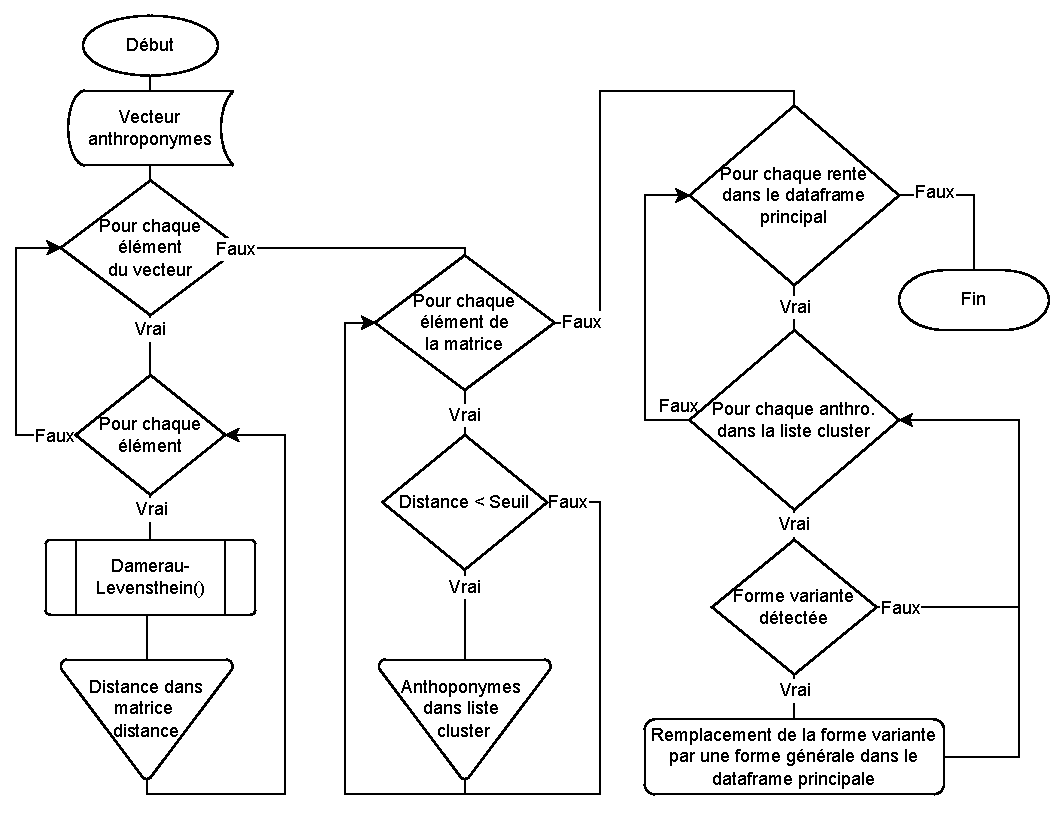
\includegraphics[scale=0.75]{2.Methods/Img/clustering.drawio.pdf} 
    \caption{Organigramme de l'algorithme de regroupement des anthroponymes}
    \label{schemaClustering}
\end{figure}



\section{Exploitation de l'information}
%draft%
Une fois les données extraient et traitées, elles peuvent finalement être exploitées.
Les phases d'exploitation de l'information  arrivent à fin du processus et vont permettre de matérialiser les objectifs de recherches.

Ces phases d'exploitation des données comprennent la modélisation des graphes planaires à partir des informations extraites et traitées, et la transposition de ces graphes en cartographie.

La modélisation des graphes planaires se fait de manière automatisée sur le logiciel Rstudio à l'aide de la bibliothèque \textit{Igraph}. Les fonctions fournit par la bibliothèque place les sommets et génère les arêtes depuis une matrice de relations et fait en sorte qu'aucune d'entre-elles ne se croisent. 

\subsubsection{Modélisation des graphes}
\subsubsection{définitions}



\subsection{Transposition des graphes en cartographie}


%résultat
\chapter{Résultats}
Ce chapitre détaillera les résultats obtenus lors de l'exécution du système pour à chacune des étapes du processus. Le système se compose d'un assemblage de scripts en langage \textit{R} appelés successivement par un programme principal dans lequel l'agent humain n'intervient à aucun moment ; il s'agit donc d'un processus entièrement automatisé. Ces scripts sont exécutés depuis le logiciel \textit{RStudio} qui est l'environnement de développement de référence pour le langage \textit{R}.

L'ensemble des scripts utilisés dans le système peut être retrouvé dans la partie \textit{Annexes} du mémoire ainsi que les résultats retournés lors de leur exécution.



\section{Segmentation du texte}
La phase de segmentation  est la première étape d'extraction des données.
L'algorithme est développé sur les vingts premières pages du registre. Lorsque celui-atteint une précision suffisante sur ce set de données réduit, il est alors testé et évalué sur l'ensemble du registre.

Lorsque le document source est importé dans l'environnement de développement en format texte (\textit{.txt}), ce dernier va découper le contenu textuel en petites chaînes de caractères au niveau des espaces et stocker celles-ci dans un vecteur de type caractère. Ceci présente l'avantage que chaque mot ou marqueur de structure peut être désigné par sa position à l'intérieur du vecteur. Par conséquent, capturer une section spécifique du texte, nécessite uniquement de pouvoir déterminer les positions du début et de fin de celle-ci au sein du vecteur.  

Le document source est donc transformé en un vecteur \textit{T} de 15390 éléments.
Quant aux procédés de détection et de capture des différentes parties du document source, ils peuvent être décrits par les expressions régulières et les formules contenues dans le tableau \ref{regexSeg}.
\vspace{0,5cm}
\renewcommand{\arraystretch} {1.5}
\begin{table}[ht]
    \centering
    \begin{tabular}{|l|c|l|}
        \hline Objet & Symbole & Regex ou Formule \\
        \hline \hline Marqueur d'escroete & $mEs$ & /\textasciicircum[IV]+([1-9])?\$/ \\
        \hline Section d'escroete & $sEs$& $ sEs_{[n]} =  T[mEs_{[n]}:mEs_{[n+1]}-1] $\\
        \hline  Définition d'escroete & $dEs $& $ dEs_{[n]} = T[mEs_{[n]}:mCo_{[1]}-1] $\\
        \hline  Marqueur de connétablie & $mCo$ & /[0-9]+°/ \\
        \hline Section de connétablie & $sCo $& $sCo_{[n]} =  sEs[mCo_{[n]}:mCo_{[n+1]}-1] $\\
        \hline Définition de connétablie & $dCo$ & $ dCo_{[n]} = sEs[mCo_{[n]}:mRdV_{1]}-1] $\\
            & & $ dCo_{[n]} = sEs[mCo_{[n]}:mRe_{1]}-1] $ \\
        \hline  Marqueur de rang de voie & $mRdv$ & /\textasciicircum[AB]\$/ \\
        \hline Section de rang de voie & $sRdv$ &$ sRdv_{[n]} = sCo[mRdv_{[n]}:mRdv_{[n+1]}-1] $\\
        \hline Marqueur de rente & $mRe$ & /[0-9]\{2,\}./ \\
        \hline Section de rente & $sRe$& $sRe_{[n]} = sRdv[mRe_{[n]}:mRe_{[n+1]}-1]$ \\
            & &  $ sRe_{[n]} = sCo[mRe_{[n]}:mRe_{[n+1]}-1]$ \\
        \hline
    \end{tabular}
    \caption{Formules et expression régulières pour la segmentation du registre}
    \label{regexSeg}
\end{table}
\vspace{0,5cm}

\subsection{Évaluation}
\subsection{Correction}

\section{Reconnaissance des entités nommées}
La reconnaissance des entités nommées s'effectue au sein des sections correspondant aux textes des rentes qui sont stockées dans le tableau de données principal. Chacune de ces sections est fouillée à l'aide d'une expression régulière afin de détecter les caractéristiques morpho-syntaxiques correspondant aux anthroponymes du  nord  de la France au Moyen-Âge.

L'expression régulière dont il est question nous est donnée par les travaux de S. De Valeriola. \\
 $/[:upper:][:lower:]+ (((l[aei']s?|d[euo']l?u?|au?)?)\{0,2\} ?[:upper:][:lower:]+(-[:upper:][:lower:]+)?)\{1,3\}/$\footfullcite[p.10]{de_valeriola_lordinateur_2021}

Celle-ci peut être décomposée en trois sous-expressions, correspondant chacune à une partie de l'anthroponyme \parencite{de_valeriola_lordinateur_2021}.
\begin{itemize}
    \item La première, $/[:upper:][:lower:]+ /$, capture le nom de baptême de la personne.
    \item La seconde , $/(((l[aei']s?|d[euo']l?u?|au?)?)\{0,2\} ?/ $ permet, quant à elle, de capturer les éventuelles particules de patronyme ( par exemple : <<de>>, <<dou>>, <<le>>, <<l'>> , <<de le>>, etc.).
    \item Finalement,  la dernière partie , $ /[:upper:][:lower:]+(-[:upper:][:lower:]+)?)\{1,3\}/ $  sert à capturer le reste du patronyme, sans les éventuelles particules.
\end{itemize}

Grâce à cette RegEx, la fonction \textit{str\_extract\_all()} du package \textit{StringR} nous retourne 799 formes distinctes d'anthroponyme. 


\subsection{Regroupement des anthroponymes}
Comme  il en a été discuté dans le chapitre \textit{Méthodes}, le choix de la méthode et de la distance de seuil pour le regroupement des anthroponymes est une étape aussi critique que délicate.
Afin de choisir la stratégie la plus adéquate, des tests on été effectués sur les 100 premiers anthroponymes, noms de baptême et patronymes recensé à travers le registre.

A travers ces tests, il a été essayé d'observer la dispersion des couples,corrects et incorrects, déterminés par l'algorithme en fonction de la distance, l'évolution du taux de bruit en fonction de la distance, et l'impact, positif ou négatif, d'une modification de pondération des opérations\footnote{Cette modification de pondération s'ajoute à celles évoquées dans le chapitre \textit{Méthodes} provenant de l'article de \fullcite[p.14]{de_valeriola_lordinateur_2021}} dans le calcul de la distance.
Cette modification de pondération consiste à passer le poids des opérations de substitution de 1,0 à 1,25. 
L'idée derrière cette modification est d'alourdir significativement le score lorsque plusieurs opérations de substitution son utilisées. 
Étant donné que la plupart des variants morphologiques d'un anthroponymes consistent en l'ajout ou la suppression d'une lettre ou d'une particule, les opérations de substitution sont relativement rare et ont un impact plus lourd que les autres opération sur la modification de la chaîne caractères.

La distance Damerau-Levensthein  entre chaque éléments testés a été calculée et tous les couples d'éléments dont la distance était égale ou inférieure à la distance de seuil (changeante en fonction de la nature des éléments testés) ont été retenus dans un tableau de données. Après quoi, chaque couple a été manuellement vérifié et annoté <<correct>> ou <<incorrect>> par l'agent humain.

Six configurations ont donc été analysées :
\begin{itemize}
    \item sur l'anthroponymes complet (nom de baptême + patronyme), considéré comme une seule chaîne de caractères, avec une distance de seuil à 3.
    \item Sur l'anthroponymes complet, avec une distance de seuil à 4, et avec avec la modification de la pondération
    \item Sur le nom de baptême uniquement, avec une distance de seuil à 2.
    \item Sur le nom de baptême uniquement, avec une distance de seuil à 2, et avec la modification de pondération.
    \item Sur le patronyme uniquement, avec une distance de seuil à 3.
    \item Sur le patronyme,avec une distance de seuil à 3, et avec la modification de pondération.
\end{itemize}


\section{Extraction des relations}
L'extraction des relations est une nouvelle phase d'extraction de l'information. Celle-ci ne peut avoir lieu qu'après la normalisation des graphies variantes des anthroponymes, qui résulte de la phase de regroupement des anthroponymes.
Le registre des rentes ayant été préalablement découpé en rentes, l'objectif de cette opération consiste à déterminer les liens qui unissent les différents individus détectés au sein d'un énoncé de rente.

Les énoncés des rentes présentent un certain formalisme dans leur structure. Nous pouvons y retrouver le motif suivant dans la presque totalité : 
\begin{enumerate}
\item L'objet de la rente +  \textbf{anthroponyme du débiteur de la rente}
\item << \textbf{ki siet entre}>> ou une variante proche de cette expression
\item <<le tènement>> +  \textbf{anthroponyme du premier voisin } + << d'une part>> 
\item << et le tènement >> + \textbf{anthroponyme du second voisin} + << d'autre part>>
\end{enumerate}
Des expressions \textit{<< ki fu >> + anthroponyme} peuvent également apparaître dans ce motif juste après un anthroponyme. Celle-ci semble désigner l'ancien propriétaire de la propriété bâtie ou du tenement. A 24 reprises,à la fin de l'énoncé de la rente, apparaissent également,  les formules <<\textit{Si fu li}>> ou <<\textit{Si fu cist}>>, suivies d'un montant et d'un anthroponyme. Le sens exact de cette partie de l'énoncé nous échappe, mais il semble --- au vu du verbe <<fu>>,  qui correspond à une forme du passé du verbe \textit{être} --- évident qu'elle n'indique pas l'individu mentionné comme voisin du débiteur de la rente. Afin de ne pas créer des relations erronées entre les individus, les énoncés des rentes seront nettoyés de ces expressions.

%nettoyage
Dans un premier temps, la colonne du tableau de données principal contenant les énoncés de rentes est copiée dans un nouveau vecteur <<\textit{rentes}>> afin de ne pas altérer les données de référence. Ensuite, de sorte qu'il ne reste plus que les anthroponymes du débiteur et de ses voisins, les rentes sont nettoyées des éventuelles expressions évoquant les anciens propriétaires grâce à la fonction \textit{str\_remove()} et à l'assemblage des deux expressions régulières suivantes : 
\[ \boxed{ 
    \text{ki fu(rent)? ((femm?e )|((le )?maistre )|((le )?vallés ))? }
    }
\]
\[ \boxed{ 
    \text{ 
        (MGR )?[:upper:]{2,} (((L[AEI']S?|D[EUO']L?U?|AU?)?){0,2} ?[:upper:]\{2,\}(-[:upper:]\{2,\})?)\{1,3\} }
    }
\]



%explication regex
La première capture l'expression <<\textit{ki fu}>> et sa forme au pluriel <<\textit{ki furent}>> ainsi que les éventuels titres ou statuts de <<femme>>, <<maistre>> ou <<vallés>> qui, s'ils ne sont pas pris en compte, bloquent la seconde expression régulière. La seconde expression régulière est celle de la détection des anthroponymes écrite par S. De Valeriola, adaptée au cas des lettres capitales.

Après cela vient la suppression des expressions <<\textit{Si fu}>> grâce à l'expression régulière suivante : 
\[ \boxed{ Si \;fu.*\$} \]
Celle-ci capture la chaîne de caractères <<\textit{Si fu}>> ainsi que tous les caractères suivant jusqu'à la fin de l'énoncé de la rente.

Lorsque les énoncés de rentes sont allégés des anthroponymes non pertinents, il est alors possible de segmenter ces énoncés en deux sous-chaînes de caractères autour des expressions <<\textit{Si sient}>>, <<\textit{Si siet}>>, <<\textit{ki sient}>>, <<\textit{ki iet}\footnote{Cette variante provient très certainement d'une erreur de typographie ou d'\textit{OCR}}>>.

À cette fin, la fonction \textit{str\_locate()} est utilisée avec l'expression régulière :
\[ 
    \boxed{
        \text{
            (S|s|K|k)i s?ien?t
        }
    }
\]
 Cette dernière nous retourne les indices dans la chaîne de caractère (de l'énoncé nettoyé) auxquels correspondent le début et la fin de l'expression recherchée. Ces indices de localisation permettent alors d'extraire une sous-chaîne de caractères depuis l'énoncé de la rente à l'endroit voulu, grâce à la fonction \textit{str\_sub()}.
 
 Lorsque les deux sous-chaînes sont récupérées, une reconnaissance des anthroponymes est effectuée dans chacune d'elles  et permet d'obtenir l'anthroponyme du débiteur dans la première, et celui de ces voisins dans la seconde. Ces relations peuvent alors être mises sous la forme de couples dans un nouveau tableau de données.
 
 \begin{figure} % insère une figure ici (h = "here")
    \centering
    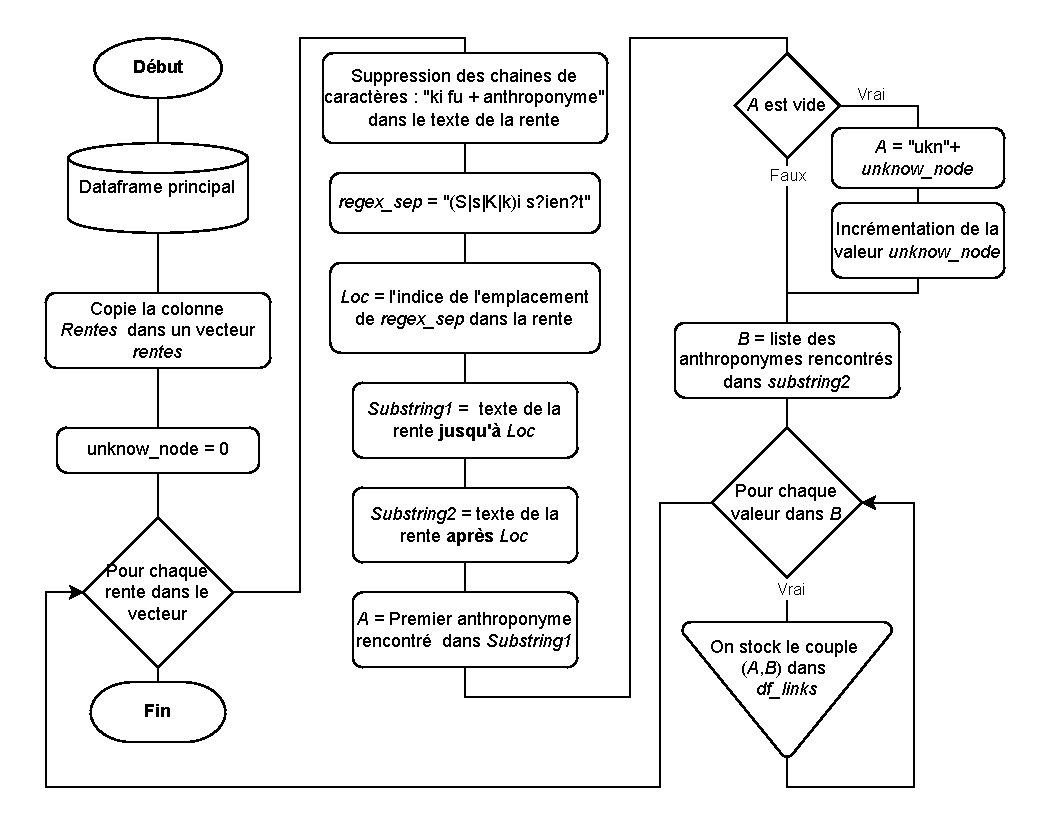
\includegraphics[scale=0.75]{3.Results/Img/rel.drawio.pdf}
    \caption{Organigramme de l'algorithme d'extraction des relations}
    \label{schemaRelations}
\end{figure}

 \begin{figure} % insère une figure ici (h = "here")
    \centering
    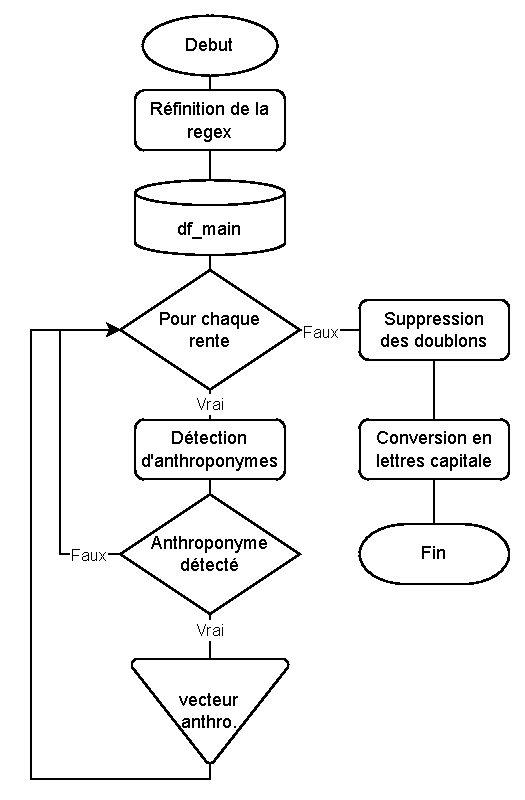
\includegraphics[scale=0.75]{3.Results/Img/clean_df_links.drawio.pdf}
    \caption{Organigramme de l'algorithme de nettoyage des paires}
    \label{schemaNettoyageRelations}
\end{figure}
 
 À la fin de cette opération, nous récupérons  un tableau de données contenant 499 couples. Parmi ceux-ci, nous observons 14 valeurs \textit{ukn} distinctes, affectant un total de 30 couples.

\subsection{Lever l'inconnue des valeurs manquantes}
Cependant, ces valeurs inconnues ne sont pas une fatalité. La commande R suivante nous permet de trouver les lignes dont il est question.
\[ df\_links[str\_detect(df\_links\$To,'ukn'),]\]
 
 Grâce aux anthroponymes connexes à la valeur inconnue, l'agent humain est dans la possibilité de retrouver les valeurs manquantes avec une recherche plein texte depuis le document source. L'analyse de ces valeurs manquantes permet de corriger certains couples qui auraient créé des erreurs dans la modélisation des graphes,  mais elle peut aussi permettre de comprendre les facteurs qui ont engendré cette perte d'information, et amener à leur correction. Le tableau \ref{ukn_node} regroupe les informations récupérées sur les valeurs manquantes après une investigation manuelle. Sur les 15 valeurs inconnues, 10 peuvent être corrigées. Nous constatons aussi que, à l'exception du \textit{Ukn11}, toutes proviennent d'irrégularités du document source. Dans une grande partie de ces cas, l'irrégularité fait que l'expression régulière ne détecte pas l'anthroponyme (comme lorsqu'il y a uniquement un nom de baptême et aucun patronyme), dans l'autre partie des cas, l'individu débiteur n'est pas clairement désigné dans l'énoncé de la rente ou  n'est simplement pas une personne (par exemple : L'ospital des Wés).
\begin{table}
    \centering
    \begin{tabular}{|l|l|l|l|}
\hline	\textbf{Ukn}	&	\textbf{Correspondance}	&	\textbf{Rente}	& \textbf{Raison}		\\
\hline
\hline	Ukn0	&	Lotin	&	5.5	&	Pas de patronyme	\\
\hline	Ukn1	&	Robiert	&	13.7	&	Pas de patronyme	\\
\hline	Ukn2	&	\textit{NA}	&	18.1	&	Pas de débiteur identifié	\\
\hline	Ukn3	&	les 2 sereurs des Lices	&	20.3	&	Sobriquet , qualificatif ou fonction	\\
\hline	Ukn4	&	le prestre des Charteriers	&	32.2	&	Sobriquet, qualificatif ou fonction	\\
\hline	Ukn5	&	Godin	&	44.3	&	Pas de patronyme	\\
\hline	Ukn6	&	\textit{NA}	&	74.12	&	Pas de débiteur identifié	\\
\hline	Ukn7	&	\textit{NA}	&	81.6	&	Pas de débiteur identifié	\\
\hline	Ukn8	&	des Carterier et des Malades	&	95.3	&	Sobriquet , qualificatif ou fonction	\\
\hline	Ukn9	&	Hamiel	&	103.	&	Pas de patronyme	\\
\hline	Ukn10	&	Daniel	&	140.5	&	Pas de patronyme	\\
\hline	Ukn11	&	Mariien de l'Eve	&	150.3	&	Anthroponyme non détecté par la RegEx	\\
\hline	Ukn12	&	Marien	&	151.4	&	Pas de patronyme	\\
\hline	Ukn13	&	L'ospital des Wes	&	206.4	&	N'est pas un anthroponyme	\\
\hline	Ukn14	&	\textit{NA}	&	244.3	&	Pas de débiteur identifié	\\
\hline
    \end{tabular}
    \caption{Valeurs manquantes dans le tableau des relations}
    \label{ukn_node}
\end{table}


\subsection{Corrections supplémentaires}
Les rentes étant classées selon un ordre topographique, il est régulier qu'un même anthroponyme apparaisse dans l'énoncé de deux ou trois rentes successives : une première fois, comme voisin d'un bien arrenté, une seconde fois, comme débiteur de la rente suivante, et une troisième fois, à nouveau comme voisin d'un autre bien arrenté adjacent au sien. Après avoir identifié les individus derrière les valeurs manquantes, il peut donc être également  intéressant de vérifier la rente précédente  et la rente suivante de chacun de ceux-ci ; au besoin, ajouter les relations  au tableau de données. Le tableau \ref{tab:corr_relation} indique les relations qui ont été incorporées au tableau de données après l'analyse manuelle des rentes précédentes et suivantes à celle d'où provenaient les valeurs manquantes.
\begin{table}
    \centering
    \begin{tabular}{|l|c|c|}
    \hline
    \textbf{N° de rente} & \textbf{From} & \textbf{To} \\
    \hline
    \hline	12.6	&	ROBIERT	&	ROBIERT DE FIERIN	\\
    \hline	14.8	&	TENEMENT DES MALADES	&	BAUDE L'ARTISIEN	\\
    \hline	139.4	&	DANIEL	&	JEHAN LE GIERMAIN	\\
    \hline	149.2	&	MARIIEN DE L'EVE	&	PIERON DE HASNON	\\
    \hline	151.4	&	MARIIEN DE L'EVE	&	MARIEN	\\
    \hline	152.5	&	MARIEN	&	MARGOT DE MAGNI	\\
    \hline
    \end{tabular}
    \caption{Relations ajoutées au tableau de données}
    \label{tab:corr_relation}
\end{table}
 
\section{Modélisation des graphes}
\subsection{Modes de représentation}
Il existe différents modes pour la représentation des objets que sont les graphes. Les trois principaux sont :
\begin{itemize}
    \item La liste <<origine/destination>> des liens,
    \item La matrice d'adjacence,
    \item La graphe sous sa forme graphique.
\end{itemize}

Ces trois formes sont équivalentes, dès lors, pour modéliser un graphe sous sa forme graphique, il est possible d'utiliser, soit une liste des liens, soit une matrice d'adjacence. La figure \ref{fig:representation_graphes}\footfullcite[p.5]{beauguitte_graphes_2010} illustre ces trois modes. Dans notre cas, nous utilisons la liste de liens  <<origine/destination>> qui est assemblée lors de la phase \textit{d'extraction des relations}, qui est la méthode la plus conventionnelle.
\begin{figure}
    \centering
    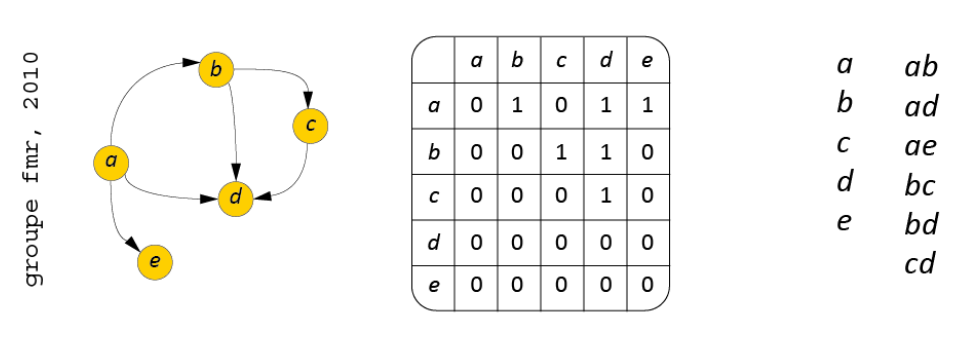
\includegraphics[scale=0.75]{3.Results/Img/mode_de_representation_graphes.png}
    \caption{Trois modes de représentation pour un même objet}
    \label{fig:representation_graphes}
\end{figure}

\subsection{Création de l'objet Igraph et modélisation}
La modélisation des graphes se fait par la fonction  \textit{graph\_from\_data\_frame()}, de la bibliothèque \textit{Igraph}, avec en paramètre le tableau de données \textit{df\_links}.
Cette fonction convertit le tableau de données introduit  en un objet Igraph  reprenant toutes les caractéristiques du graphe. Cet objet peut ensuite être traduit en visualisation en employant la fonction de base \textit{plot()} ou \textit{ggraph()}.

\begin{figure}[h]
    \centering
    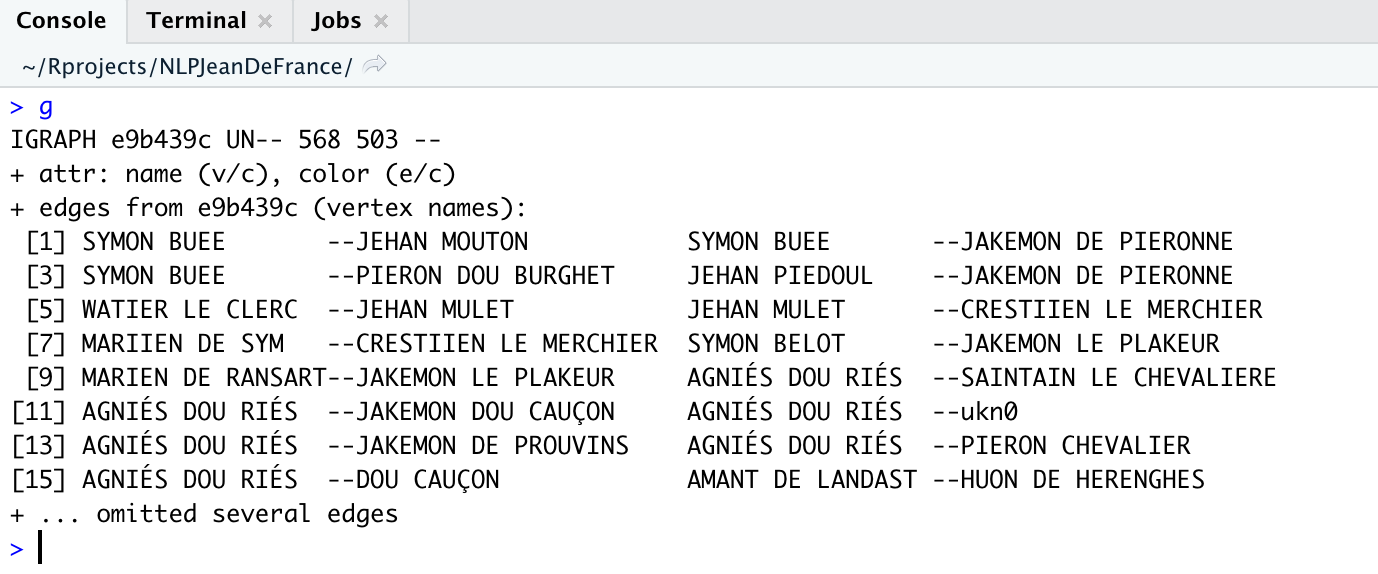
\includegraphics[scale=0.50]{3.Results/Img/igraph_object.png}
    \caption{Objet Igraph convertible en visualisation graphique}
    \label{fig:objetIgraph}
\end{figure}

% premier exemple
Un premier essaie avec les paramètres par défaut, sur un ensemble choisi aléatoirement de cinq rentes successives\footnote{Il s'agit des rentes 19.2 , 20.3, 21.4, 22.1 et 23.2 } nous donne le résultat de la figure  \ref{fig:test_graphe}.

\begin{figure}[h]
    \centering
    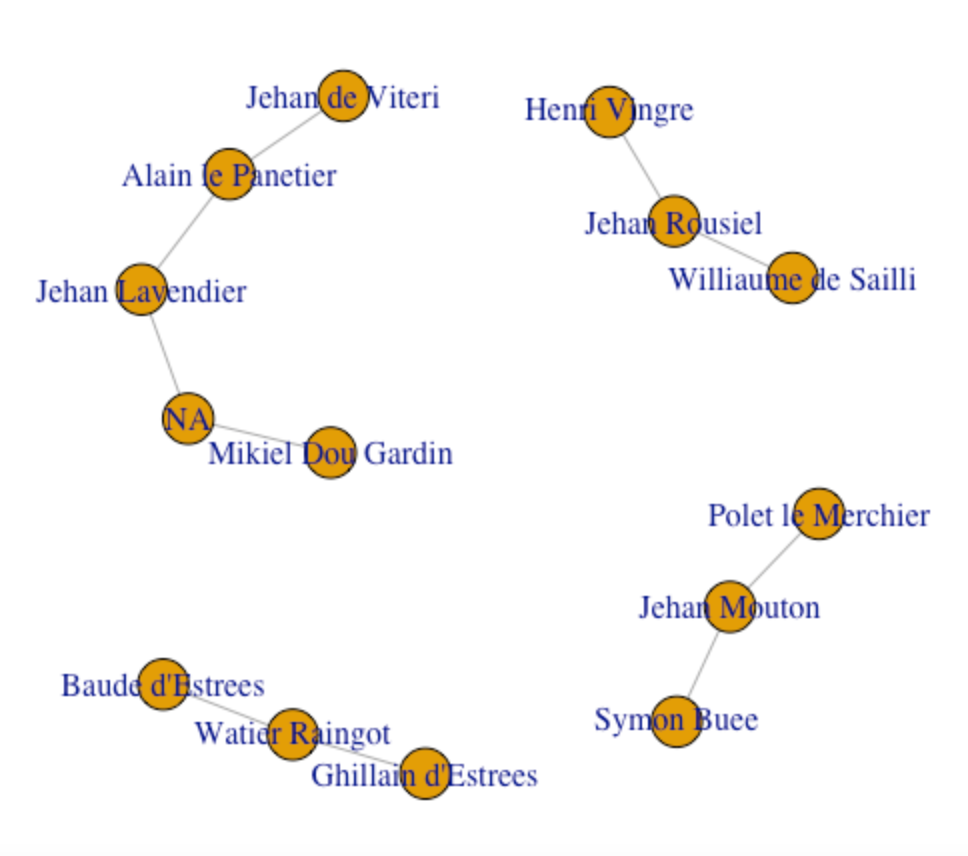
\includegraphics[scale=0.45]{3.Results/Img/graphe_test.png}
    \caption{Graphe des relations mitoyennes, généré sur base des rentes 19.2 à 23.2 }
    \label{fig:test_graphe}
\end{figure}

%modélisation
Lorsque le graphe comprend un nombre important de sommets, comme dans  notre cas, il est plutôt désigné comme \textit{grand graphe} ou comme \textit{grands réseaux}. Cela implique de devoir adapter les paramètres  de la fonction qui modélise le  graphe, sous peine que ce dernier ne devienne illisible par le chevauchement des sommets, des arêtes ou des labels.

Par rapport au premier graphe de la figure \ref{fig:test_graphe}, la taille des sommets a donc été réduite et les labels des sommets ont été supprimés, à l'exception de celui de Jehan de Franche. Également,  une couleur a été affectée à chaque arête en fonction de l'escroete contenant la relation. Pour finir, la spatialisation, c'est-à-dire,  l'algorithme qui définit l'emplacement des sommets dans le plan, est définie par le paramètre \textit{layout}. Pour générer le graphe de la figure  \ref{fig:plot_igraph}, c'est le layout \textit{layout\_nicely} qui a été sélectionné. Ce layout tente de déterminer lui-même la spatialisation la plus appropriée. À ce stade, les sommets sont encore placés de manière non déterministe : chaque appel de la fonction \textit{plot()}  générera un graphe différent, et ce, bien que les paramètres soient inchangés. Cette visualisation nous permet toute foi d'avoir un premier regard  sur la connectivité  des sommets, la longueur des chemins et leur localisation au niveau des escroetes.

\begin{figure}
    \centering
    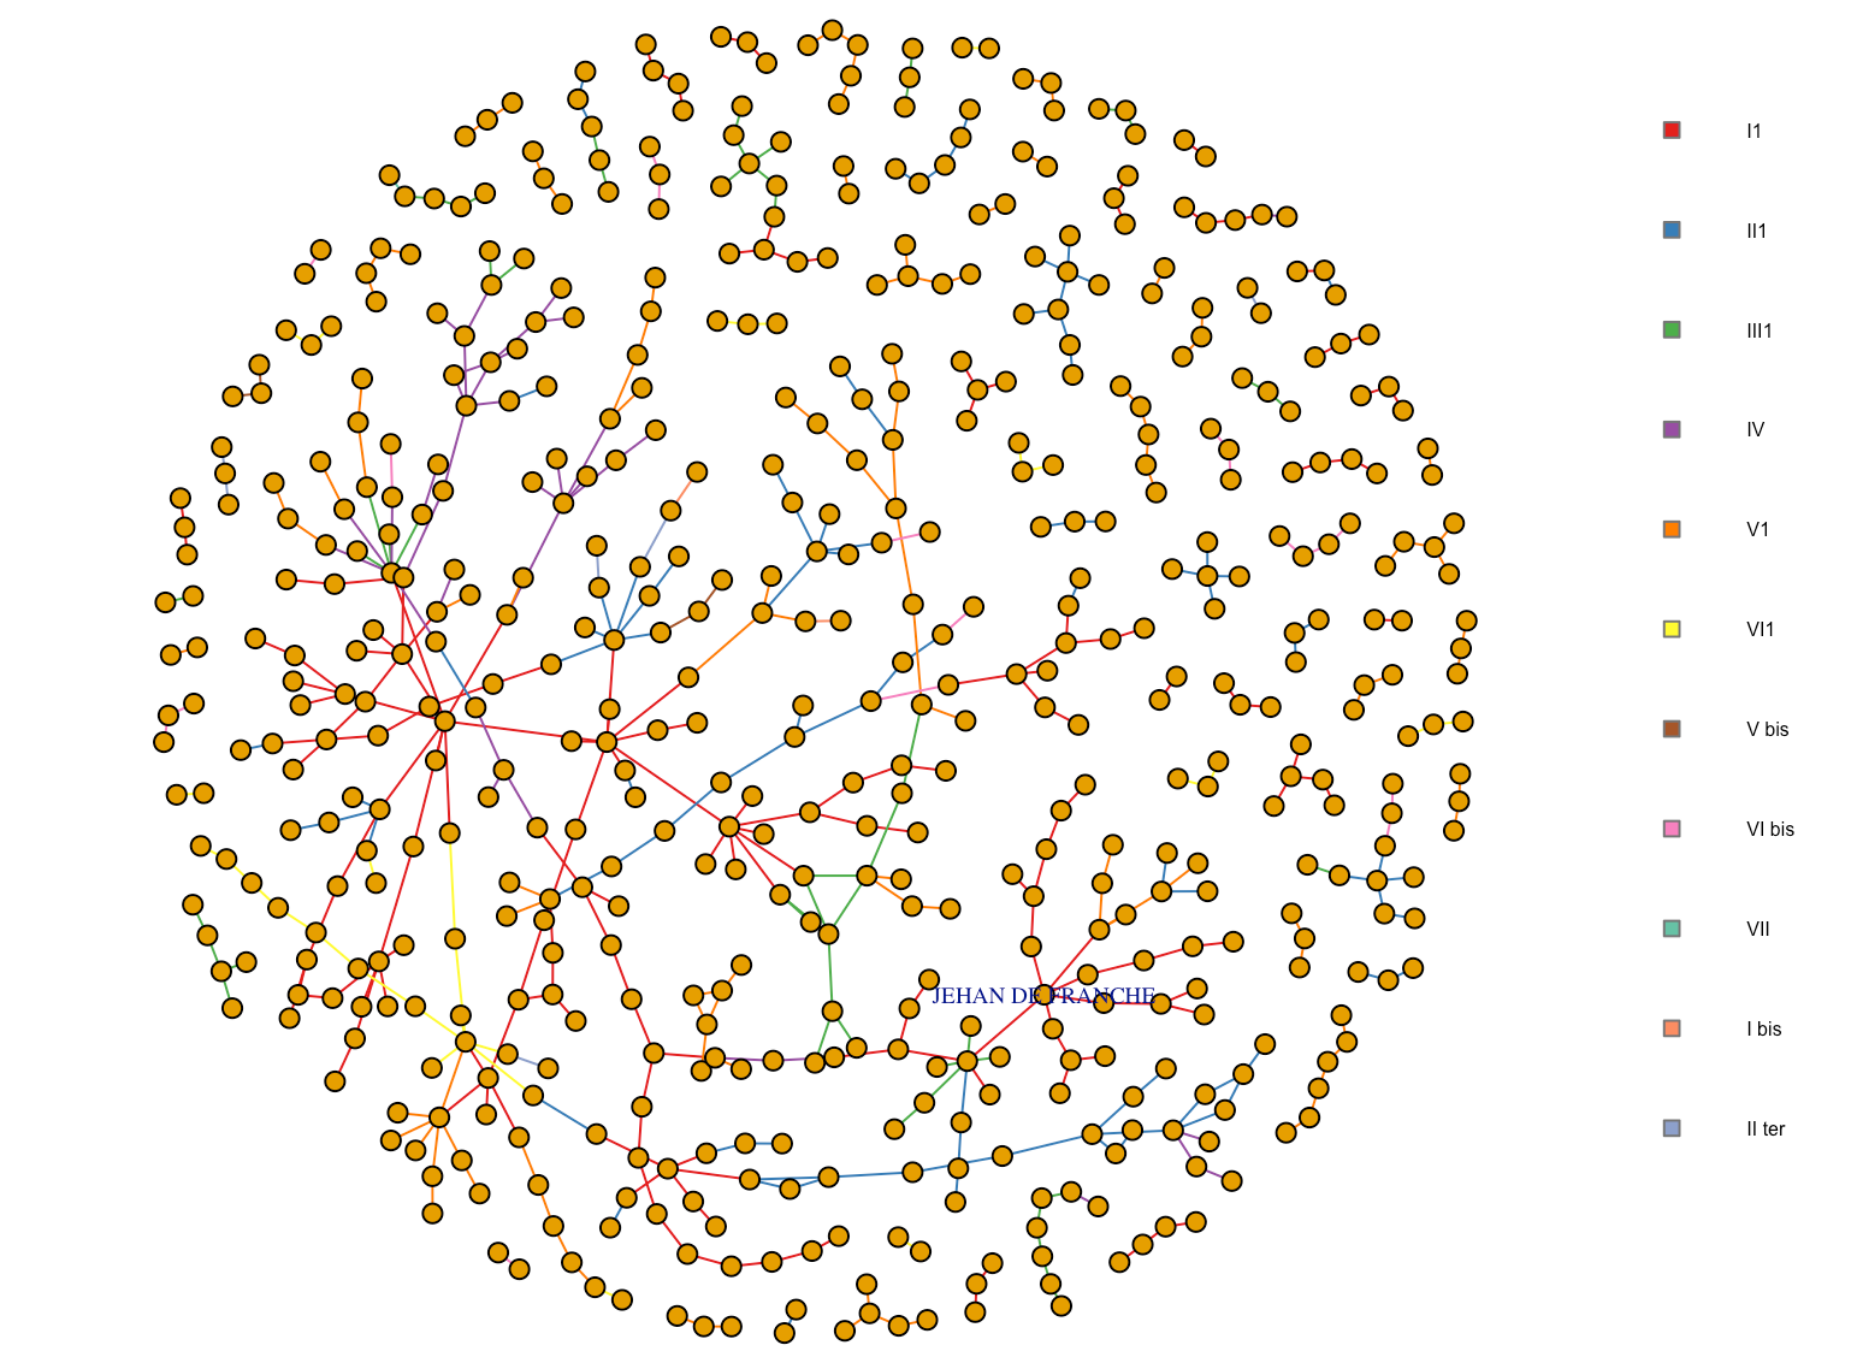
\includegraphics[scale=0.45]{3.Results/Img/plot_igraph.png}
    \caption{Graphe des relations mitoyennes, généré sur base de la fouille de texte automatisée dans le registre de rentes de Jean de France }
    \label{fig:plot_igraph}
\end{figure}

D'autres algorithmes de spatialisation ont été testés, mais aucun ne s'est révélé réellement plus pertinent comme le montre la figure \ref{fig:layout}.

\begin{figure}
    \centering
    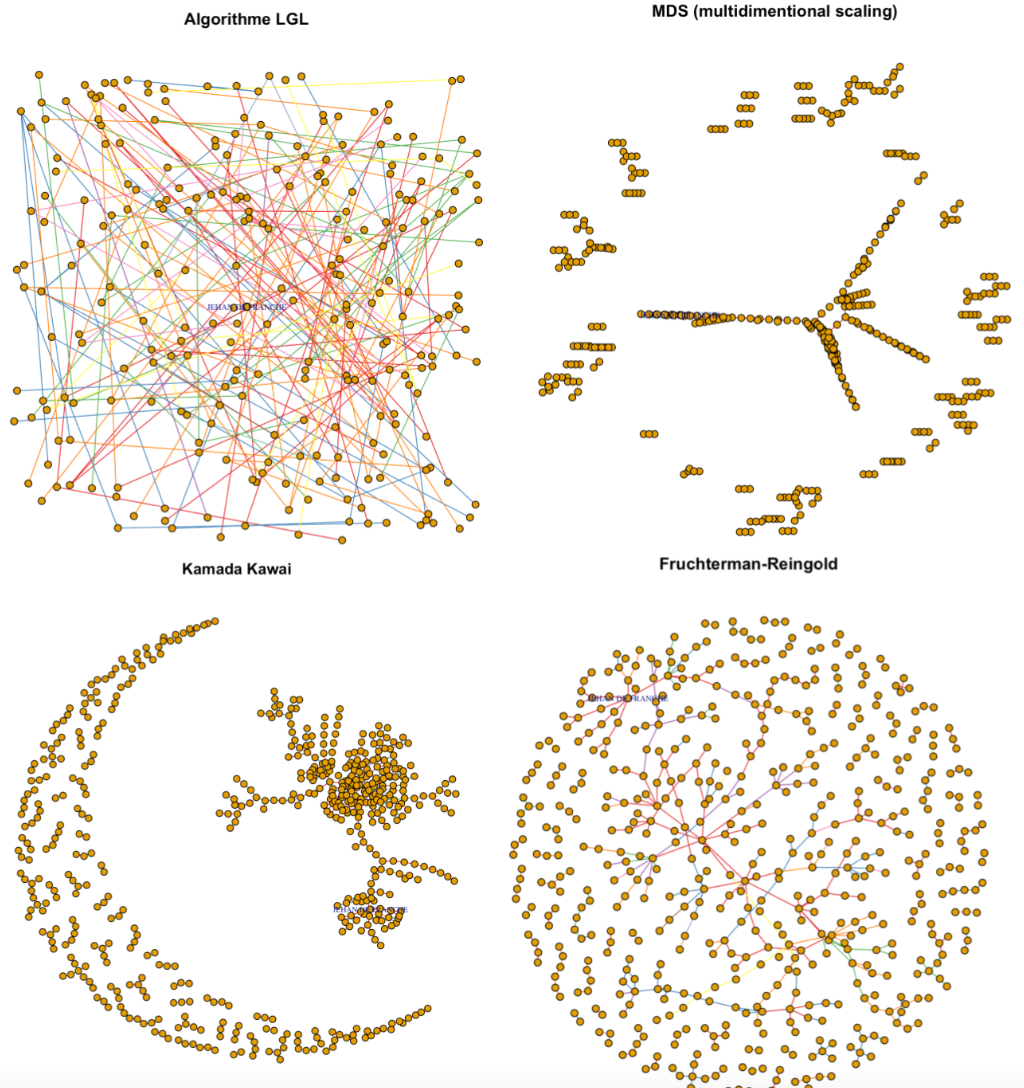
\includegraphics[scale=0.5]{3.Results/Img/layout.png}
    \caption{Différents algorithmes de spatialisation}
    \label{fig:layout}
\end{figure}

\section{Transposition des graphes en cartographie}





%discussion
\chapter{Discussions}
Ce chapitre se consacre à la mise en perspective des résultats obtenus par le système développé et à leur confrontation aux objectifs initialement déclaré afin de valider ou d'invalider l'hypothèse émise dans le chapitre \textit{introduction} de ce mémoire. Il y sera aussi abordé les difficultés et limites rencontrées, ainsi que des pistes de solutions ou d'améliorations envisageables.
\section{Difficultés rencontrées}
%difficulté document historique

\subsection{La complexité du document historique}
Le travail s'est heurté aux difficultés inhérentes à toutes études de documents historiques. Ces difficultés peuvent  être partagées en deux catégories : celles intrinsèques au contenu du document et celles issues du support du document. 

Dans la première catégorie, se retrouve les problèmes d'incompréhensions et de confusions liés au vocabulaire, aux glissements sémantiques aux variantes de graphies, ou à la langue utilisée \parencite{piotrowski_natural_2012}.
Notre document, le rentier de Jean de France, est écris en picard médiéval ; une langue relativement proche de l'ancien français. De part ses racines, cette langue possède de grandes ressemblances avec notre français contemporain et permet par conséquent, dans une certaine mesure, une compréhension relative de celle-ci à n'importe quel profane francophone.
Cependant, cette compréhension sommaire ne permet pas d'appréhender les aspects plus subtils de la langue et la signification de certaines formulations reste donc très supposées. 

L'exemple le plus parlant de cette difficulté est le traitement de l'expression << ki fu >> que l'on retrouve abondamment dans le registre. Tout du long de travail, cette expression a été considérée comme le marquage de l'ancien propriétaire de la maison ou du tenement. Mais cela n'est ni plus ni moins, qu'une supposition issue de déductions personnelles et n'est étayée par aucune source. Il se pourrait que l'expression aient plusieurs sens selon sa position dans la phrase : qu'elle désigne l'ancien propriétaire lorsqu'elle est placé devant l'anthroponyme \footnote{ << \textit{Sour le  maison Mgr Sauwalon de Vregelai et sur tout le tenement, \textbf{ki fu Adam le Linnier}} >>} dans le sens << qui fût à >> et que lorsqu'elle est placée après  un anthroponyme, prend le sens de  << qui fût >>, <<feu(e)>>\footnote{ << \textit{Sour 2 maisons \textbf{Daniel, ki fu} clers le le bailliu} >> }. A nouveau, il ne s'agit là que d'interprétations personnelles mais aucune documentation n'a été trouvée afin de répondre à ces questions. Par conséquent, une partie du travail à du s'accomplir dans un spectre d'incertitude avec la réflexion et l'esprit critique pour seuls outils.

La seconde catégories regroupe les difficultés issue du support du document. 
En l'occurrence, notre document est passée d'un format physique en papier en documents texte par plusieurs étapes intermédiaires, chacune entraînant une série d'altérités du document original (erreurs de typographie, d'\textit{OCR}, de transcription , etc...). \footnote{L'historique du document ayant été  largement traité dans le chapitre \textit{Méthodes}, nous n'enterons pas plus dans le détail dans cette partie-ci.}

\subsection{L'enjeux de la qualité des données}
L'autre principal obstacle auquel le travail s'est confronté, est la dégradation progressive de la qualité des données.
La stratégie adoptée, qui s'appuie sur l'utilisation d'expressions régulières offre l'avantage de permettre une automatisation des processus sans avoir à recourir aux approches orientées connaissance ou aux approches orientées données. Néanmoins, elle dévoile aussi certain inconvénients : sa forte rigidité face aux exceptions rencontrées et la fragilisation du système que cela implique. Tous les cas possibles doivent être anticipés et préparés car la moindre irrégularité dans la forme des données traitées entraîne, au mieux, une perte de données, au pire, la corruption d'autres données. Dans le cas de données semi-structurées et non-structurées telles que celles extrait du registre de rentes cela s'avère donc relativement délicat. Bien que le registre soit organisé et présente un certain formalisme dans les énoncés de ces rentes, on y trouve encore de nombreuses d'irrégularités, nous forçant à adapter le code à chacune d'elles. 

La phase de segmentation retourne un ensemble de données relativement correct et suffisant pour poursuivre les phases suivantes.

C'est à partir de là, que la qualité des données commence à diminuer, et ce, pour plusieurs causes.

Dans un premier temps, on retrouve des erreurs arrivées dans le tableau de données lors de la segmentation, celles-ci trouvent parfois leurs origines dans le document source lui-même, comme lorsqu'il s'agit d'erreurs de typographie, d'\textit{OCR}.
Dans d'autres cas, il s'agit des algorithmes qui ne sont pas parfaitement adaptés et qui capturent une chaîne de caractères tronquée ou inadéquate après avoir rencontré une irrégularité dans la morphologie d'une expression, d'un noms ou d'une formule.
Ces erreurs peuvent ensuite se répercuter dans le reste du système. Certaines sont bénignes, mais d'autres vont s'amplifier au fur et à mesure du processus et finir par causer d'importantes pertes de données. 

Ensuite, on retrouve une perte de la qualité des donnés suite au tronquage de celles-ci. Comme il en a déjà été discuté, nous avons estimé le silence moins néfaste que le bruit, dès lors, une partie des données s'est vu être tronquée afin de réduire le risque d'assimiler des données fausses ou conflictuelles. A nouveau, ces pertes d'informations peuvent possiblement en entraîner d'autres, car parmi les données rejetées, certaines auraient potentiellement pu servir à enrichir le tableau de données des sommets. Au terme du processus, même s'il s'agit d'un choix délibéré, on ne peut que déplorer la perte de cette quantité de données.

Il est assez difficile d'évaluer l'impact réel qu'à pu avoir cette diminution progressive de la qualité des données sur les résultats finaux obtenus en sortie du système. Celle-ci n'a pas été le facteur le plus limitant quo a été rencontré, mais reste,  sans équivoque, un enjeux prépondérant.

\subsection{Problèmes mineurs rencontrés}

Quelques autre problèmes ont été également rencontrés. Ils ont des répercussions moindre par rapports à ceux discutés précédemment, mais il convient tout de même de les évoquer.

Tout d'abord, l'observation de différents tableaux et du graphe a permis de mettre en évidence  qu'un même individu pouvait être débiteur de plusieurs biens. Un aspect de la réalité qui, bien qu'il puisse paraître évidement, a été négligé lors du développement et qui engendre des erreurs ponctuelles dans le graphe (toutes les occurrences d'un même anthroponyme étant modélisé par un unique sommet, alors que ces dernier sont censés correspondre à un emplacement géographique précis).
Une erreur de compréhension du document source et du contexte étudié, qui est finalement  symptomatique des difficultés évoquées plus haut.
Malgré cela, le graphe n'ayant pas été transposé sur le fond de carte et la règle définie pour l'enrichissement du tableau de données des sommets, ces erreurs n'ont pu avoir que assez peu d'incidence. 

Un second problème mineur rencontré est celui des ressources cartographiques disponibles. D'une part, une alternative opensource à du être employée suite à la tarification de l'\textit{API} de \textit{Google Maps}. Malheureusement, le catalogue de cette alternative ne propose pas de fonds de cartes de haute résolution pour la région de Douai. D'autre part, il ne semble pas exister de fond carte << historique >>, or la topographie des lieux à drastiquement changé depuis le Moyen Âge.
\section{Pistes d'améliorations}
Le mémoire décrit le développement d'un système traduisant un document historique textuel en cartographie. Le processus par lequel passe le document est long  et traverse nombreux champs des technologie de l'information et des humanités numériques. Dans le cadre de ce  mémoire, qui est avant tout un prototype, un \textit{proof of concept}, ces aspects n'ont pu être explorés que dans une profondeur relative, voire de manière très superficielle pour certain. De fait, les pistes d'amélioration du système sont très nombreuses.

\subsection{Nettoyage des erreurs d'\textit{OCR} et de typographies}
%intro
Dans cadre de ce mémoire, une retranscription du registre de rentes en format  \textit{word(.docx)} a été fournie par % ...%. 
.Cette retranscription est relativement propre et contient assez peu d'erreurs résiduelles d'\textit{OCR} ou de typographies. Elle était donc utilisable sans qu'il faille passer par une phase de correction préalable. S'il avait fallu utiliser une version provenant directement de l'\textit{OCRisation} du livre de G.Espinas, ce nettoyage aurait été très certainement nécessaire. 

La correction des erreurs d'\textit{OCR} se base généralement sur des approches statistiques nécessitant des corpus de la langue cible. Si l'on considère l'approche d'utiliser uniquement les données provenant du livre, qui a caractérisé l'intégralité du travail, je suggère une stratégie similaire à celle adoptée pour le regroupement des anthroponymes.

%analyse des besoins%
L'entièreté du texte n'a pas besoin d'être corrigé pour être utilisable, mais seulement certaines expressions servant à la reconnaissance de la structure du texte par les algorithmes d'extractions de l'information ainsi que les valeurs (les erreurs au sein des noms d'entités nommées sont, en toute logique, corrigées lors de la phase de regroupement des anthroponymes). Dans les expressions liées à la structure du texte, on retrouve par exemple l'expression <<\textit{ki sient entre}>> (et ses variantes), qui dans le texte sépare le débit-rentier de ses voisins ou  les expressions <<\textit{dou fond de la tiere}>> et <<\textit{aprés le fond de la tiere}>>  qui permettent d'identifier le montant et la nature de la rente à verser au débit-créancier, tandis que dans les <<valeurs>> on va retrouver les différentes utilisées pour régler le payement, par exemple % ... %.

%stratégie%
Je suggère donc de créer manuellement une liste de ces différentes expressions. Et une fois le fichier importé dans \textit{RStudio} et son contenu textuel transformé en un vecteur, de fusionner les éléments par petits groupes en fonction de l'expression que l'on cherche à corriger (par cinq pour l'expression <<\textit{ki sient entre}>> par exemple). 
Ensuite, calculer la distance Damerau-Levensthein\footnote{La distance Damerau-Levansthein sans les modifications de pondération apportées dans le cadre du regroupement des anthroponymes} entre l'expression testée et tous les éléments du vecteur, puis à remplacer par l'expression testée, ceux dont la distance est inférieure à un seuil préétabli. %exemple en annexe%
%conclusion
Cette stratégie nécessiterait un temps de calcul considérable mais présenterait l'avantage d'être automatisée et de ne nécessiter aucune ressource extérieures.

\subsection{Mise en place d'un système de table de données}
%système de table de données
\subsection{Amélioration de la qualité des données}
%amélioration de la qualité des données
\subsubsection{Regroupement des anthroponymes}
Comme déjà discuté, le regroupement d'anthroponymes est une problématique complexe qui ne trouve actuellement aucune solution générale parfaite dans la littérature. Il est par conséquent nécessaire d'apporter des modifications à ces solutions imparfaites pour les rendre plus adéquates au spécificités du contexte étudié.

Afin d'améliorer la méthode employée, il a été envisagé de coupler le calcul de distance avec des éléments extraient lors de la segmentation tels que le numéro de rente ou la connétablie. Cette idée nait  de deux constats.
Le premier est que les rentes sont, pour la quasi totalité, classées dans le registre selon un ordre topographique. Le second, est qu'une fois les rentes nettoyées des expressions <<ki fu + anthroponyme>> (et de leurs variantes), les personnages sont, à priori, mentionnés, soit en tant que de débitrentier habitants des propriétés faisant l'objet de la rente, soit en tant qu'habitant des propriétés mitoyennes à la rente. Par conséquence, une même personne ne devrait pas être mentionnée dans différentes rentes éloignées géographiquement. 
Malheureusement, cette hypothèse se voit être réfutée par l'analyse du graphe  qui nous montre des sommets avec des degrés très élevé, jusqu'à 10 pour \textit{Richart Pourciel}\footnote{Une recherche en \textit{plein texte} dans le document source nous confirme qu'il y a effectivement des mentions de cet individu dans différentes connétablies et qu'il ne s'agit pas d'une erreur d'un des algorithmes}.
De cela, découle deux suppositions qui devront être considérées afin de diminuer les erreurs au sein du système. 
\begin{itemize}
    \item Certain de personnage peuvent être débiteur de plusieurs rentes immobilière. 
    \item Plusieurs individus partagent le même anthroponyme, soit des cas d'homonymies.
\end{itemize}

Une autre approche pour améliorer la reconnaissance et regroupement d'anthroponymes serait de coupler avec d'autres sources ou base de données et d'envisager une stratégie orientée connaissance.
Finalement, il reste toujours la possibilité d'améliorer l'algorithme de calcul des distances en modulant le poids des opérations dans des cas précis (diminuer le poids de l'ajout ou de la suppression d'un espace pour alléger le score des particules dans les patronymes, par exemple). Ceci nécessite d'effectuer de nombreux essaies et analyses qui sont lourdes en terme de ressources informatiques\footnote{Pour calculer les distances séparant chacune des 799 formes d'anthroponymes capturées entre-elles, l'ordinateur a travaillé pendant presque une heure}, mais l'informatique quantique, qui se fait de plus en plus accessible via des options de \textit{cloud computing}, devrait améliorer notablement la vitesse d'exécution de ce type de calcul. 

\subsubsection{Enrichissement des  données}
\subsection{Extension du projet}
%montant des rentes
%dispersion des patronymes
%évolution de l'empire immobilier de JdF  en couplant l'avec l'analyse des actes notariés du livre de G.Espinas
%amélioration du code
\section{Conclusion}
Les objectifs fixés au départ ayant été partiellement atteints, il semble compliqué de donner verdict tranché concernant les résultats obtenus. 

Plusieurs aspects doivent être nuancés et prêtent à discutions.
Commençons avec celui de l'automatisation du processus.
Deux interventions de l'agent humain ont été nécessaires : la première consistait en la correction du regroupement des anthroponyme tandis que la seconde consistait à trouver les correspondances entre les éléments topographiques du XIIIe siècle et les éléments topographiques actuels. 

Cela étant, l'automatisation totale d'un tel système, sans plus de ressource, semble utopique. En effet, s'il est concevable qu'un algorithme destiné à regrouper les différentes graphies d'anthroponymes sur performe celui nous avons utilisé et permet, ainsi, une entière automatisation de cette partie du système, il l'est beaucoup moins que l'on puisse automatiser la seconde intervention. Celle-ci est déjà relativement complexe lorsqu'elle est exécuté manuellement par l'homme parce qu'elle requiert un travail de recherche approfondi au sein de multiples sources non-structurées ainsi qu'une réflexion critique à l'égard de ces dernières.

Un second aspect qu'il convient d'évoquer est le changement de méthodes et d' objectifs intervenu lors de la dernière phase. Fondamentalement, l'objectif a toujours été de d'inscrire sur la carte les demeures des différents individus cités dans le registre, et en ce sens, les cartes produites rentrent dans ce cadre. Cette première perspective, qui suggérait de transposer le graphe sur le fond de carte, en cherchant à profiter que les maisons  soient décrites par leurs attenances dans le registre, afin de reconstituer les allées des rues, est finalement un usage assez peu conventionnel de l'analyse de réseau. Par conséquent, le projet c'est heurté à une contrainte technologique où les outils utilisés n'étaient pas en mesure de répondre aux besoins de cette approche. Au lieu de cela, le graphe a été utilisé de sorte à déterminer les informations topographiques de certains sommets à partir de celles  des sommets voisins. 

Cependant, si l'objectif initial n'est pas totalement atteint, il n'en demeure que les cartographies produites ne sont pas dénuées d'intérêts. Elles permettent une approche visuelle des données textuelles contenue dans le registre de rentes. De plus, les différents graphes et tableaux de données créés pour parvenir à ces cartographies, ont eux aussi leur part d'intérêt. Tandis que les tableaux sont une énumération des données prélevées, les graphes, eux, matérialise les relations qui les unissent. Il en ressort une réserve d'informations structurées, exploitables en vue d'étudier différents aspect de la réalité décrite par le registre de rentes de Jean de France ou d'émettre de nouvelles de nouvelles hypothèses. Pour donner quelques exemples : le tableau de données principale peut être utilisé afin d'étudier les montants et différentes espèces de rentes en fonction des zones topographiques, tandis que le tableau de correspondance des connétablie  peut être ré-exploitée dans l'étude d'autres documents contemporains à Jean de France.
On peut supposer également que l'analyse de la densité des sous-graphe permettrait d'identifier les centres névralgiques de la ville et l'observation des connections entre sommets de connétablies différentes puisse servir à retrouver la localisation de connétablies  aujourd'hui disparue (à l'image de celles longeant les fossets ou la rue fait-en-paille).

En l'état actuel, la justesse et la précision des cartes produites sont insuffisantes pour qu'elles puissent être utilisées seules ou comme références.
Mais il ne s'agit là que d'un prototype, presque d'une étude de faisabilité. Les résultats, bien d'imparfaits me semblent déjà encourageants. Selon moi, si les différents éléments du systèmes améliorés, cette approche pourrait être adaptée à d'autres documents historiques de même nature, et devenir un outil très pertinents pour visualiser ou agréger l'information contenue dans de gros corpus de documents. 

Ceci démontrerait une nouvelle fois que les méthodes d'analyses quantitatives, bien que parfois complexes à mettre en place,  apporte une réelle complémentarité à l'étude traditionnelle des sciences humaines.
%Annexes
\begin{appendices}
\chapter{Annexes}
\begin{figure}[ht] % insère une figure ici (h = "here")
    \centering
    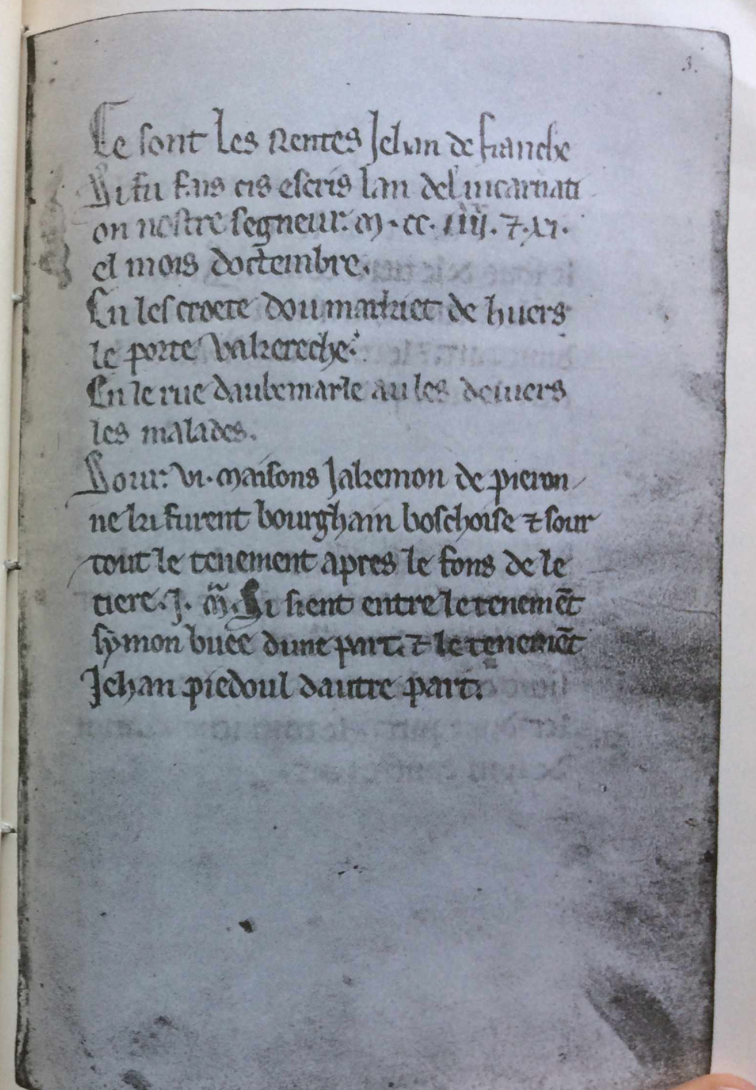
\includegraphics[scale=1]{5.Appendix/Img/escris.png} 
    \caption{Première page du registre de rente de Jean de France, photographe inconnu}
\end{figure}
\listoffigures
\listoftables
\nocite{*}
\printbibliography
\end{appendices}
\end{document}